%%%%%%%%%%%%%%%%%%%%%%%%%%%%%%%%%%%%%%%%%%%%%%%%%%%%%
%% File: main.tex
%% Author: John Liaperdos (ioannis.liaperdos@gmail.com)
%% This version JC
%% Last update: April 28, 2015
%% Description: Provides an example of a PhD Thesis 
%% using the teipel-thesis-en pdfLaTeX class.
%%
%% Character encoding: UTF-8
%%%%%%%%%%%%%%%%%%%%%%%%%%%%%%%%%%%%%%%%%%%%%%%%%%%%%
%
%
%%%%%%
% 1. use the "modern" or "classic" option to switch between 
% a modern or classic font, respectively.
%
% 2. add/remove the "hyperref" option to enable/disable hyperlinks:
% (remember to remove auxiliary files after adding/removing 
% the "hyperref" option).
%
% 3. add/remove the "printer" option to typeset a printer-friendly 
% (grayscale)/color version of the thesis.
%
% 4. use the "watermark" option to indicate a draft copy of the thesis
%
% 5. use the "histinit" option to enable "historiated initials".
% (If used, all chapter initials declared by the \InitialCharacter{}
% macro are enlarged. If ommitted, arguments of \InitialCharacter{}
% are typeset as normal text.)
%
% 6. use the "plain" option to disable tikz graphics in title page
% and part/chapter headers (might help to avoid compilation timeouts).
% Note that "plain" disables CD label and CD cover creation.
%
% 7. use the "noindex" option to (hopefully) avoid compilation timeouts
% when compiling online (disables index generation - note that "\indexGR",
% "\index" invocations need not be removed when toggling this option).
%
% 8. use the "frontispiece" option to typeset a frontispiece at the back of the cover page
%
% 9. use the `letter' option for a US letter page layout, instead of A4
%
%%%%%%%%%%%%%%%%%%%%%%%%%%%%%%%%%%%%%%%%%%%%%%%%%%%%%%%%%%%%%%%%%%%%%%%%%%%%%%%
%
	  %\documentclass[modern,hyperref,watermark,histinit,frontispiece,plain]{teipel-thesis-en}
	   \documentclass[classic, hyperref,watermark,histinit,frontispiece,plain]{teipel-thesis-en} %%moder pone el formato lindo, pero los simbolos griegos no
%
\graphicspath{{figures/}}
\usepackage[scientific-notation=true]{siunitx}
%\usepackage[spanish]{babel}
\usepackage[english]{babel}
\usepackage{graphicx, color}
\graphicspath{{figures/}}
\usepackage{amsmath}
\usepackage{amscd}
\usepackage{youngtab}
\usepackage{titlesec}
%\usepackage[latin1]{inputenc}
%\usepackage[utf8]{inputenc}
\usepackage{listings}
\usepackage{enumerate}
\usepackage{amssymb}
\usepackage{amsthm}
\usepackage{syntonly}
\usepackage{fancyhdr}
\usepackage{cancel}
\usepackage{siunitx}
\usepackage{slashed}
\usepackage{bbm}
\usepackage{dsfont}
%
\usepackage{multirow}
\usepackage{gensymb}
\usepackage{cite} % to collet the references
\usepackage{fancyhdr}
\pagestyle{fancy}
\fancyhf{}
\usepackage{dsfont}
\usepackage{float}

\usepackage{fancyhdr}
\pagestyle{fancy}
\fancyhf{}
\fancyhead[LO]{\leftmark} % En las p\'{a}ginas impares, parte izquierda del encabezado, aparecer\'{a} el nombre de cap\'{\i}tulo
\fancyhead[RE]{\rightmark} % En las p\'{a}ginas pares, parte derecha del encabezado, aparecer\'{a} el nombre de secci\'{o}n
\fancyfoot[C]{\thepage} % N\'{u}meros de p\'{a}gina en el centro

%%size
\setlength{\oddsidemargin}{-0.2 cm}
\setlength{\evensidemargin}{-0.2 cm}
\setlength{\textwidth}{16.2 cm}

%%%%%%%%%%%%%%%%%%%%%
%% UNIVERSITY INFO 
%%%%%%%%%%%%%%%%%%%%%%%%%%%%%%%%%%%%%%%%%%%%%%%%%%%%
%
% University Name
%
	\UniversityName{Universidad de Antioquia}
%
% School Name
%
	\SchoolName{Instituto de Física}
%
% Department Name
%
	\DepartmentName{Facultad de Ciencias Exactas y Naturales \\
						{\large{Grupo de Fenomenología de Interacciones Fundamentales}} }
%
% Location
%
	\UniversityLocation{Medellín}
%
%
%%%%%%%%%%%%%%%%%%%%%%%%%%%%%%%%%%%%%%%%%%%%%%%%%%%%
%% THESIS INFO 
%%%%%%%%%%%%%%%%%%%%%%%%%%%%%%%%%%%%%%%%%%%%%%%%%%%%
%
%% -------------------------------------------------------------------
% Thesis Type
%
	\ThesisType{\\PhD Thesis}
%
%% -------------------------------------------------------------------
% Thesis Title 
%
% To force line breaks in title, use "\\".
% If different line break locations are to be used for the cover page and the inner title page (page 3) 
% repeat the cover page title as an optional argument of the \title macro, including line breaks.
%
% Examples:
% 1. Automatic title line breaks in cover page and inner title page: 
%	    \title{This is my title}
% 2. Title breaking after ''my'' in both cover page and inner title page:
%	    \title{This is my \\ title}
% 3. Title breaking after ''my'' in cover page, and after ''is'' in inner title page:
%	    \title[This is my \\ title]{This is \\ my title}
%
	\title{ Título del proyecto o tesis  }
%%
%
%% -------------------------------------------------------------------
%% Thesis subtitle (optional)
%
% If no subtitle is required, set argument to blank, or comment-out the \subtitle macro.
%
% Example:
%%	\subtitle{This is my subtitle}
	\subtitle{with this subtitle}
%
%% -------------------------------------------------------------------
%
%% Author name
%
% For more than one authors, separate with ",".
% Example:
%	\authorName{Albert Einstein, George W. Bush} 
	\authorName{Juan Valdez} 
%
%% -------------------------------------------------------------------
%
%% Supervisor's name
% 
	\supervisor{Albert Einstein  }
	\cosupervisor{Richard Feynman  }
%
%% -------------------------------------------------------------------
%% Supervisor's title
%
	\supervisorTitle{}
%
%
%% -------------------------------------------------------------------
%% Place and date of publication
%
	\thesisPlaceDate{Medellín, 2018}
%
%% -------------------------------------------------------------------
%% Place and date in acknowledgements (if applicable).
%
	\ackPlaceDate{Medellín, 2018}
%
%% -------------------------------------------------------------------
%% Approval information
%
	\examinationDate{ Date:}
	\approvalStatement{Approved by \hspace{2.0 cm}}
%
%% -------------------------------------------------------------------
%% Copyright Year
%
%	\copyrightYear{Creative Commons Wikipedia-like}
%
%% -------------------------------------------------------------------
%% Name of first examiner
%
%	\firstExaminer{Professor A}
	\firstExaminer{\hspace{5.0 cm}}
%
%% -------------------------------------------------------------------
%% Title of first examiner
%
	\firstExaminerTitle{}
%
%% -------------------------------------------------------------------
%% Name of second examiner
%
	\secondExaminer{\hspace{5.0 cm}}
%
%% -------------------------------------------------------------------
%% Title of second examiner
%
	\secondExaminerTitle{}
%%
%%
%%%%%%%%%%%%%%%%%%%%%%%%%%%%%%%%%%%%%%%%%%%%%%%%%%%%%%%%%%%%%%%%%%%%%%
%% THESIS COLORS: 
%%%%%%%%%%%%%%%%%%%%%%%%%%%%%%%%%%%%%%%%%%%%%%%%%%%%%%%%%%%%%%%%%%%%%%
%%
%% Color for cover and chapters
	\chaptercolor{brown!75!magenta}
%%
%% Color for appendices
	\appendixcolor{brown!80!magenta}
%%
%% hyperlink color (ignored if the "hyperref" option is omitted)
    	\hyperlinkcolor{red!55!brown}
%%
%% Thesis title foreground color in cover page (ignored if the "plain" option is used)
    	\titlecolor{white}
%%
%% Thesis title background color in cover page (ignored if the "plain" option is used)
    	\titlebackgroundcolor{brown!85!magenta}  
%%
%%
%%%%%%%%%%%%%%%%%%%%%%%%%%%%%%%%%%%%%%%%%%%%%%%%%%%%%%%%%%%%%%%%%%%%%%
%% COVER PAGE IMAGE: 
%%%%%%%%%%%%%%%%%%%%%%%%%%%%%%%%%%%%%%%%%%%%%%%%%%%%%%%%%%%%%%%%%%%%%%
%%
%% Cover page image (optional)
%% If no cover page image is required, set argument to blank, or comment-out the \coverpageimage macro.
%%
%% Syntax:
%%          \coverpageimage{scale factor}{path to cover page image}
%%      or
%%          \coverpageimage[tikz]{scale factor}{TikZ commands}
%%          (commands may include \usetikzlibrary statements, etc.)
%%      
%% Examples:
%%      - Use the image in "figures/rdf.png" scaled by 0.8 (=80%):
%%          \coverpageimage{0.8}{figures/rdf.png}
%%      - Use a TikZ drawing scaled by 0.5 (=50%):
%%          \coverpageimage[tikz]{0.5}{
%%              \draw[thick, magenta] \foreach \x in {18,90,...,306} {
%%                  (\x:4) node{} -- (\x+72:4)
%%                  (\x:4) -- (\x:3) node{}
%%                  (\x:3) -- (\x+15:2) node{}
%%                  (\x:3) -- (\x-15:2) node{}
%%                  (\x+15:2) -- (\x+144-15:2)
%%                  (\x-15:2) -- (\x+144+15:2)
%%              };
%%          }
%%
     \coverpageimage{0.4}{figures/neutrino_mass_diagram}
     %\coverpageimage{0.3}{figures/bullet2}  
     \vspace{2.0 cm}
%%
%%
%%%%%%%%%%%%%%%%%%%%%%%%%%%%%%%%%%%%%%%%%%%%%%%%%%%%%%%%%%%%%%%%%%%%%%
%% MISCELLANEOUS SETTINGS: 
%%%%%%%%%%%%%%%%%%%%%%%%%%%%%%%%%%%%%%%%%%%%%%%%%%%%%%%%%%%%%%%%%%%%%%
%%
% Path to University Logo (all supported formats are allowed)
	%\UniversityLogoPath{logo/teikal_logo.eps}
	\UniversityLogoPath{figures/logo-udea}
%
% Path to University Logo (grayscale version to be used with the `printer' option)
	\UniversityBWLogoPath{figures/logo-udea.eps}
%
% Scalefactor for University logos (1 for 100%)
	\LogoScaleFactor{1.1}
% Draft Indication (watermark text to be used with the `watermark' option)
	\draftIndication{}%poner algo debajo de superviso en la primera hoja
%
% Frontispiece settings (ignored if the `frontispiece' option is omitted)
%	Syntax: \setFrontispiece[scale factor]{path to frontispiece image}{frontispiece image legend}
	\setFrontispiece[0.3]{figures/logo-udea}{Universidad de Antioquia} %figura detras de la primera página ---> GUITARRA
%
%%%%%%%%%%%%%%%%%%%%%%%%%%%%%%%%%%%%%%%%%%%%%%%%%%%%%%%%%%%%%%%%%%%%%%
%
% add custom hyphenation rules here
%\hyphenation{} 
%
%%%%
%
%
%%%%
\begin{document}

\maketitle

\beginfrontmatter
	
% Abstract (content in `abstract.tex')
	\begin{abstract}

En éste trabajo se estudia la sensitividad en el LHC de la producción de un $W^{\prime}$ via quarks bottom ($b$) y quarks charms ($c$), y decaimientos al sabor leptónico $\tau$ en el rango de masas de $200$ a $1000$ GeV. Aquí se muestra que el quarks $b$ necesario en el mecanismo de producción puede  mejorar la diferenciación de las señales respecto al background, en comparación con un análisis inclusivo que depende exclusivamente del  $\tau$-tagging y $E^{\text{miss}}_T$. Se presentan límites posibles en los acoplamientos y se comparan con el mejor ajuste a las anomalías en $R (D^{(*)})$ en las desintegraciones del mesón $B$. \\

   \begin{keywords}
    	LHC, Fisica de altas energías, Boson $W^{\prime}$, Anomalías de sabor.
   \end{keywords}

\end{abstract}

	%\begin{abstract}

We study the LHC sensitivity to a $W^{\prime}$ produced via bottom ($b$) and charm ($c$) quarks and decaying to  $\tau$ flavor leptons in the mass range 200-1000 GeV. We show that the extra $b$ quarks necessitated by the production mechanism can improve the background rejection compared to an inclusive analysis relying solely on $\tau$-tagging and $E^{\text{miss}}_T$. We present prospective limits on the couplings and compare them to the best fit to the $R (D^{(*)})$ anomalies in $B$ meson decays. 
   \begin{keywords}
    	LHC, High energy physics, Boson $W^{\prime}$, Flavor anomalies.
   \end{keywords}

\end{abstract}

% Dedication
	\thesisDedication{Short inspired phrase here}
% Acknowledgements (content in `acknowledgements.tex')
	%%%%%%%%%%%%%%%%%%%%%%%%%%%%%%%%%%%%%%%%%%%%%%%%%%%%%%%%%%%%%%%%%%
%%
%% use the starred version of the "acknowledgements" environment
%% to omit signatures from this section, e.g.:
%% \begin{acknowledgements*} ... \end{acknowledgements*}
%% 
%%%%%%%%%%%%%%%%%%%%%%%%%%%%%%%%%%%%%%%%%%%%%%%%%%%%%%%%%%%%%%%%%
\begin{acknowledgements}

I would like to thanks all the people that in some way have helped me with the elaboration of this thesis.

First, I would like to thanks ....
\end{acknowledgements}
% Table of Contents
	\tableofcontents
% List of Figures
	%\listoffigures
% List of Illustrations
	%\listofillustrations
% List of Tables
	%\listoftables
% Preface (content in `preface.tex') 
	%\begin{preface}
	Preface goes here ...  
\end{preface}
	
\beginmainmatter

%%%%%%%%%%%%%%%%%%%%%%%%%%%%%%%%%%%%%%%%%%%%%%%%%%%%%
%% INCLUDE YOUR CHAPTERS/SECTIONS HERE
%%
% Introduction
	\chapter{Introducci\'{o}n}
El Modelo Estándar de partículas (ME) es una teoría altamente exitosa, debido a que explica una gran cantidad de experimentos de altas energías, tanto en la frontera de energías, como de intensidad. Sin embargo, es una teoría que se considera incompleta, debido a la aparición de nuevos fenómenos los cuales no son posibles de explicar mediante este (materia oscura, energía oscura, masa de neutrinos, entre otros). Por lo que se espera que las manifestaciones de la Nueva Física (NF) o física más allá del ME, aparezcan por encima de la escala de Teraelectronvoltios (TeV), ya que hasta el momento no se ha encontrado nada a escalas menores. 

Con el inicio de operaciones del gran colisionador de hadrones (LHC, por sus siglas en inglés) a su máxima potencia, se esperaba encontrar evidencia que pudiera demostrar la existencia de nuevas partículas e interacciones que dieran solución a estos problemas, pero hasta el momento no se ha encontrado pruebas fuertes que den indicios sobre NF.

Una gran cantidad de teorías que explican NF consideran que el grupo gauge del ME $SU(3)_C \times SU(2)_L \times U(1)_Y$ está incluido en un grupo gauge más grande que al romper espontáneamente las simetrías (directamente o a través de varias etapas) cae en el grupo gauge del ME. El rompimiento espontaneo de simetrías de este nuevo grupo gauge se da en o sobre la escala de TeV, por lo que el ME es visto como un modelo efectivo válido a bajas energías. Algunos modelos que incluyen NF son: Teorías de Gran Unificación (TGU) y modelos inspirados en teorías de cuerdas~\cite{Faber:2018qon}. Curiosamente, se predicen una gran cantidad de observables cuando la última ruptura espontánea del grupo gauge extendido se produce. 

En particular, es posible poner a prueba estos modelos mediante observables de física de sabor, debido a la impresionante precisión y alcance de los experimentos actuales. Es tal la precisión, que gracias a estos se ha logrado encontrar algunas anomalías que van en contra de algunas predicciones del ME~\cite{Amhis:2014hma}. Una de las predicciones del ME es la Universalidad Leptónica (UL), ésta establece que los bosones vectoriales se acoplan por igual a las tres familias de leptones~\cite{Abazov:2007wy}. Lo que implica que dichos bosones deben decaer con igual probabilidad a las tres familias de leptones. 

Las mediciones de los decaimientos $b \rightarrow c \ell \nu$ para diferentes leptones de estado final, pueden ser utilizadas para probar la UL con una gran precisión, dado la cancelación de muchas fuentes de incertidumbres teóricas que ocurren en relaciones, tales como:
\begin{align}
R(D^{(*)}) = \frac{\Gamma(B \rightarrow D^{(*)} \tau \nu)}{\Gamma(B \rightarrow D^{(*)} \ell \nu)}\,,
\end{align}
con $\ell = e$ o $\mu$. BaBar, Belle y LHCb han observado  anomalías en la UL. Los últimos promedios medidos para estos procesos son $R(D) = 0.397 \pm 0.049$ y $R(D^*) = 0.316 \pm 0.019$~\cite{Aaij:2014ora}, lo cual implica una desviación combinada de $4 \sigma$ respecto al valor del ME. Adicionalmente, las mediciones de la razón
\begin{align}
R_K = \frac{\Gamma(B \rightarrow K \mu ^+ \mu ^-)}{\Gamma(B \rightarrow K e^+ e^-)}\,,
\end{align}
realizadas por la colaboración LHCb muestran una desviación de $2,6 \sigma$ del valor registrado para el ME, $R_K = 0,745 ^{+0,090} _{-0,074} \pm 0,036$~\cite{Aaij:2014ora}. 

Si estos observables se convierten en una prueba de la no UL, sería lo que muchos físicos interpretan como la primera señal firme de la existencia de física más allá del ME en la escala electrodébil~\cite{Hiller:2003js,Guevara:2015pza,Bordone:2016gaq}.
Igualmente se han detectado anomalías en la distribución angular en las observaciones del decaimiento $b \rightarrow s \mu ^+ \mu ^-$. Ajustes globales realizados a $b \rightarrow s \ell ^+ \ell ^-$ por diferentes grupos muestran una buena concordancia y una explicación coherente para obtener NF de estos valores anómalos del ME con significancias alrededor de $4 \sigma$ ~\cite{Descotes-Genon:2013wba,Horgan:2013pva,Ghosh:2014awa,Hurth:2014vma,Altmannshofer:2014rta,Altmannshofer:2015sma,Descotes-Genon:2015uva,Hurth:2016fbr}. Mientras que en el caso de los observables de $b \rightarrow s \mu ^+ \mu ^-$ la cuestión de las incertidumbres hadrónicas todavía plantea algún debate~\cite{Beaujean:2013soa,Descotes-Genon:2015uva,Jager:2014rwa,Hurth:2014vma,Lyon:2014hpa,Ciuchini:2015qxb}. 

El esfuerzo de los físicos de partículas teóricos se ha centrado en el estudio de diferentes modelos que permitan explicar dichas anomalías en el decaimiento del mesón $B$. Principalmente se han desarrollado modelos que pueden explicar sólo una de las anomalías: ya sea $R(D^{(*)})$ o $R_K$. Los modelos que explican ambos conjuntos de anomalías son más escasos. Esto se debe a la dificultad de diferenciar las contribuciones de procesos que poseen un tamaño similar y  que tienen lugar en el ME en órdenes diferentes: nivel de loop para $R_K$ y nivel de árbol para $R (D^{(*)})$.  En ese sentido es necesario estudiar modelos que permitan una posible explicación a ambas anomalías.

Una posible solución a las anomalías en el decaimiento del mesón $B$, son los modelos con dos dobletes de Higgs (2HDM, por sus siglas en ingles) tipo III  ~\cite{Chen:2017eby,Iguro:2017ysu}. En los modelos tipo III ambos dobletes de Higgs se acoplan a todos los campos fermiónicos, lo que permite corrientes neutras que cambian el sabor a nivel árbol. Igualmente, este modelo permite obtener un Higgs cargado después de rompimiento espontáneo de simetría. Dicho estado es utilizado como una corriente cargada, mediante la cual se da explicación a las anomalías expuestas anteriormente. Además, es posible establecer que el estado de Higgs cargado decaiga en leptones cargados y neutrinos, permitiendo posibles señales de detección en aceleradores modernos~\cite{AristizabalSierra:2006ri}.
Otra posible solución consiste en explicar las anomalías en términos de bosones de gauge extras a los del ME~\cite{Boucenna:2016wpr}. En este caso se adicionan bosónes vectoriales $Z^{\prime}$ y $W^{\prime}$, considerando que el grupo gauge del ME está embebido en un grupo gauge mayor, de la forma $SU(3)_C \times SU(2)_1 \times SU(2)_2 \times U(1)_Y$. Gracias a que estos bosones gauge se pueden producir en los aceleradores del LHC, es posible establecer restricciones de los acoples de estos directamente a los quarks de la primera generación. Estos acoples suelen tener fuertes restricciones con los datos actuales. Sin embargo, si dichos bosones se acoplan poco a las partículas de las primeras generaciones, esto es favorable, ya que las anomalías de sabor usualmente están asociadas con partículas de la tercera generación.

En este trabajo nos centraremos en tratar de dar explicación a las anomalías de sabor mediante la introducción de un nuevo bosón vectorial cargado $W^{\prime}$ al ME. Este bosón permite dar explicación a las diferentes anomalías con una corriente cargada implicada, por lo que es necesario generar nuevas señales de producción de  dicho bosón que puedan ser observados en experimentos actuales de física de altas energías. Por lo que el objetivo principal será desarrollar nuevas técnicas de búsqueda, que permitan dilucidar dichas anomalías. 

El resto de este documento está organizado de la siguiente manera: En el capítulo \ref{Ch:W} se describen las propiedades más importantes del bosón $W$. En el capítulo \ref{Ch:W-prime} se describe las interacciones del bosón $W^{\prime}$ y sus propiedades más relevantes. En el capítulo \ref{Ch:results} se presentan los resultados y se hace un analisis de estos. En el capítulo \ref{Ch:Conclusiones} se presentan las conclusiones y resumen de los resultados.

% Parts/Chapters
%	\part{Part A}
\chapter{Bosón $W$}\label{Ch:W}
En el año 1933, Fermí presenta al mundo su teoría original de la desintegración beta~\cite{Fermi:1933jpa}, en esta los procesos son tratados como interacciones de contacto, las cuales se producen en un único punto, es decir, no se requiere de partículas intermediarias. Debido a que la interacción débil (la responsable de la desintegración beta) es de muy corto alcance, la suposición propuesta por Fermí es acertada y produce excelentes resultados a bajas energías. Sin embargo, debido a los desarrollos teóricos de la época se sabía que a altas energías esta aproximación no era útil y por lo tanto se debía crear una teoría en la cual la interacción estuviera mediada por alguna partícula. Algunos físicos teóricos propusieron una partícula intermediaría que llamaron bosón  vectorial intermediario~\cite{Lee:1960qw}. A partir de allí el desafío para lo físicos teóricos era predecir las propiedades del bosón vectorial intermediario, y para los experimentales, producir este en el laboratorio.
Debido a que no había un modelo o teoría que diera información formal sobre el bosón vectorial intermediario, las conjeturas sobre su masa se fueron refinando a medida que los experimentos aumentaban progresivamente la energía. En 1965 se creía que la masa debía ser al menos masa del protón~\cite{Kienzle:1965zz}; 10 años después, el límite inferior experimental creció a $2.5$ veces la masa del protón~\cite{Kramer:1970ed}. Sin embargo, fue necesario esperar hasta la aparición de la teoría electrodébil de Glashow, Weinberg y Salam. Esta teoría daba argumentos firme sobre el valor de dicha masa. De hecho, en esta teoría hay tres bosones vectoriales intermedios, dos de ellos cargados ($W^{\pm}$) y uno neutral ($Z$). Las predicciones dadas por la teoría electrodébil establecía que las masas de estos bosones vectoriales intermedios debía ser~\cite{Weinberg:1967tq}:
\begin{align}
M_{W} =& 82 \pm 2 \text{ GeV/c}^2\,, & M_{Z} =& 92 \pm 2 \text{ GeV/c}^2\,.
\end{align}

De la teoría electrodébil se conocía que todos los hadrones y leptones participan en la interacción débil, pero debido a que dicha interacción solo es relevante en ausencia de las interacciones fuertes y electromagnéticas, la masa de estos bosones vectoriales intermediarios es difícil de medir. La dificultad fue superada debido a la construcción del colisionador protón-antiprotón Super Proton Synchrotron (SPS, supersincrotrón de protones) del CERN~\cite{Arnison:1983mk, Arnison:1983rp}, mediante el cual fue posible producir estas partículas extremadamente pesadas (la masa del protón es de $1 \text{ GeV/c}^2$, por lo que estos bosones vectoriales intermediarios son casi $100$ veces más pesados que el protón). En enero de 1983, el grupo de Carlo Rubbia informó sobre el descubrimiento de los $W$ (a $81.5\text{ GeV/c}^2$) y en junio, el mismo grupo anunció el descubrimiento del $Z$ (a $95.3 \text{ GeV/c}^2$)~\cite{Rubbia:1984xy}. Esto significo un extraordinario triunfo técnico y de fundamental importancia para la comunidad de física, ya que, poder determinar las masas de los bosones $W$ y $Z$ permitía probar la consistencia interna del ME.

\section{Interacción débil}
La interacción débil es generada por la carga débil, lo cual les permite a las partículas con carga débil la interacción con los bosones $W$ y $Z$. En el caso del $W$ la interacción es un cuadrivector  y se acopla a una cuadricorriente $j^{\mu}_w$ (corriente débil $H_W = g_W j^{\mu}_w W_{\mu}$) la cual es generada por el movimiento de las partículas portadoras de carga débil ( es decir, quarks y leptones). La constante de acoplamiento $g_W=\sqrt{4\pi \alpha_W}$ es la constante de acople débil. Primero estudiaremos la interacción del $W$ con los leptones. Dicha interacción es determinada por el vértice leptónico fundamental, el cual se presenta en la figura~\ref{Fig:lvtoW}.
%
\begin{figure}
\centering
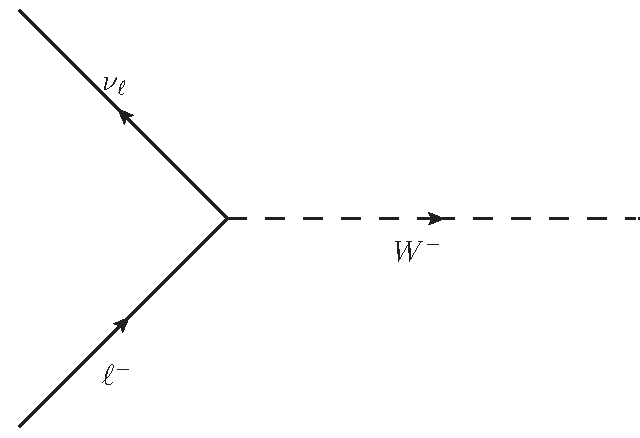
\includegraphics[scale=0.67]{lvtoW.pdf}
\caption{Vértice leptónico fundamental}
\label{Fig:lvtoW}
\end{figure}
%
Aquí un leptón ($e$, $\mu$ y $\tau$) es convertido en su correspondiente neutrino ($\nu_e$, $\nu_{\mu}$ y $\nu_{\tau}$), con la emisión de un $W^{-}$ (o la absorción de $W^{+}$). El proceso de convertir un neutrino en leptones también está permitido y los procesos cruzados incluyen los antileptones. La importancia de las corrientes cargadas en la interacción débil es que permiten cambiar sabor, a diferencia de las demás interacciones que no lo permiten. La regla de Feynmann para el vertice de la interacción débil está dado por:
%
\begin{align*}
\frac{-i g_{W}}{2\sqrt{2}} \gamma^{\mu}(1-\gamma^5)\,,
\end{align*}
%
el factor $2\sqrt{2}$ es por convención,  y el factor ($1-\gamma^5$) hace referencia a que las corrientes débiles solo se acoplan a los leptones levógiros o izquierdos, lo que permite la violación de la simetría de paridad (P).

El acoplamiento de los $W^{\pm}$ se da estrictamente solo para una generación de leptones en particular:
%
\begin{align*}
\begin{pmatrix}\nu_e \\ e \end{pmatrix} \,, &
&\begin{pmatrix}\nu_\mu \\ \mu \end{pmatrix} \,, &
&\begin{pmatrix}\nu_\tau \\ \tau \end{pmatrix} \,.
\end{align*}
%
Los únicos procesos permitidos son $e^{\pm} \to W^{\pm} + \nu_e$, $\mu^{\pm} \to W^{\pm} + \nu_\mu$ y $\tau^{\pm} \to W^{\pm} + \nu_\tau$. Estas restricciones se deben a las leyes de conservación del número electrónico, el número muónico y el número tauónico. El acoplamiento de $W$ a quarks no es tan simple, porque aunque la estructura de generación es similar
%
\begin{align*}
\begin{pmatrix}u \\ d \end{pmatrix}\,, & 
&\begin{pmatrix}c \\ s \end{pmatrix}\,, &
&\begin{pmatrix}t \\ b \end{pmatrix}\,,
\end{align*}
%
las interacciones débiles no está estrictamente restringidas entre generaciones. Debido a que hay interacción entre las partículas de la misma genereación, por ejemplo $d \to u + W^{\pm}$. Pero existen también procesos que combinan generaciones de la forma $s \to u + W^{\pm}$. Si este no fuera el caso, tendríamos tres leyes absolutas de \textquotedblleft conservación del sabor\textquotedblright: la conservación de \textquotedblleft upness-plus-downness\textquotedblright, \textquotedblleft encanto-más-rareza\textquotedblright y \textquotedblleft verdad-más-belleza\textquotedblright análogas a las tres leyes de conservación del número leptónico. De hecho, si así fuera, la partícula extraña más ligera ($K^-$) sería absolutamente estable, y también lo sería el mesón $B$ (la partícula hermosa más liviana); el universo sería un lugar diferente a lo que se conoce.

En 1963, cuando solo se conocían los quarks $u$, $d$ y $s$, el físico Italiano Nicola Cabibbo propuso que los vértices de las interacciones de los quarks debían ser corregidos~\cite{Cabibbo:1963yz}. El vértice $d + \bar{u} \to W^{-}$ debía ser corregido por un factor de $\cos \theta_C$ y el vértice $s + \bar{u} \to W^{-}$ por un factor de $\sin \theta_C$, donde $\theta_C=0.226$ rad es conocido como el ángulo de Cabibbo. Debido a su pequeño valor el vértice $s + \bar{u} \to W^{-}$ está más suprimido que el vértice $b + \bar{u} \to W^{-}$, lo que indica que a diferencia de la interacción débil para leptones, la interacción débil para quarks no prohíbe la interacción entre generaciones~\cite{Cabibbo:1963yz}.
%
\begin{figure}
\centering
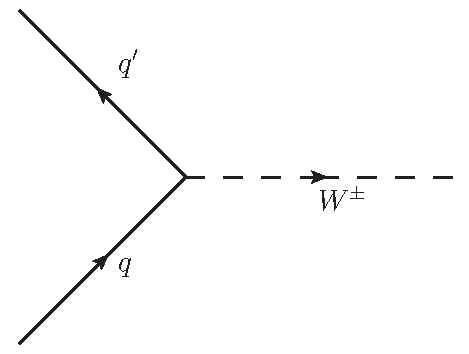
\includegraphics[scale=0.8]{qqtoW}
\caption{Vértices de interacción del bosón $W$ con los quarks. $q$ y $q'$ hacen referencia a los diferentes sabores de quarks ($u$, $d$, $c$, $s$, $b$ y $t$).}
\label{Fig:qqtoW}
\end{figure}
%
La teoría de Cabibbo fue muy exitosa reproduciendo resultados experimentales de una gran cantidad de decaimientos, pero surgió un problema: bajo este modelo la amplitud de decaimiento del mesón $K^{0}$ en un par $\mu^{+}\mu^{-}$ calculada es mucho mayor que los límites experimentales permitidos debido al proceso de la fig.~\ref{Fig:Ktomumu}, el cual es proporcional a $\sin \theta_C \cos \theta_C$. Una solución a este problema fue propuesto por Glashow, Iliopoulos y Maiani (GIM)~\cite{Glashow:1970gm}. Esta solución fue nombrada como mecanismo de GIM, este mecanismo consiste en introducir un cuarto quark (quark $c$), para el cual el vértice de la interacción $c + \bar{d} \to W^{-}$ lleva un factor de $-\sin \theta_C$ y el vértice $c + \bar{s} \to W^{-}$ lleva un factor de $\cos \theta_C$. Debido a este nuevo quark el proceso de la fig.~\ref{Fig:Ktomumu} es cancelado por el diagrama con el mismo proceso intercambiando el $u$ con el $c$, el cual será proporcional a $-\sin \theta_C \cos \theta_C$.

Una simple interpretación de este mecanismo consiste en que los estados físicos de los quarks deben ser $d'$ y $s'$, en lugar de  $d$ y $s$, dados por:
%
\begin{align}\label{Eq:Rot}
\begin{pmatrix}d' \\ s' \end{pmatrix} =& \begin{pmatrix}\cos \theta_C & \sin \theta_C \\ -\sin \theta_C & \cos \theta_C \end{pmatrix}\begin{pmatrix}d \\ s \end{pmatrix} \,.
\end{align}
%
Los bosones $W$ se acoplan a los estados de “Cabibbo rotados”
%
\begin{align*}
\begin{pmatrix}u \\ d' \end{pmatrix}\,, & 
&\begin{pmatrix}c \\ s' \end{pmatrix}\,,
\end{align*}
%
de la misma forma en que se acoplan al par de leptones; donde el acople a las partículas físicas están dados por:
%
\begin{align*}
\begin{pmatrix}u \\ d' \end{pmatrix} =& \begin{pmatrix}u \\ d\cos \theta_C + s \sin \theta_C \end{pmatrix}\,, & 
\begin{pmatrix}c \\ s' \end{pmatrix} =& \begin{pmatrix}c \\ -d\sin \theta_C + s \cos \theta_C \end{pmatrix}\,.
\end{align*}
%
Lo cual implica que $u + \bar{d} \to W^{-}$ lleva un factor de $\cos \theta_C$, $u + \bar{s} \to W^{-}$ lleva un factor de $\sin \theta_C$, $c + \bar{d} \to W^{-}$ lleva un factor de $-\sin \theta_C$ y $c + \bar{s} \to W^{-}$ lleva un factor de $\cos \theta_C$. \footnote{Es de notar que la elección del uso de los quarks tipo down ($d$ y $s$) es una definición arbitraria y por convención. Esto no representa una asimetría física entre quarks de tipo up ($u$ y $c$) y tipo down. Por lo que un desarrollo que  describa los estados de la interacción débil $u'$ y $c'$, en términos de $u$ y $c$ es totalmente equivalente.} El mecanismo GIM se consideraba extravagante debido a que para dar solución a un defecto técnico bastante esotérico, debía introducir un nuevo quark. Además,  para la epoca gran parte de esta teoría estaba aun sin probar. En 1974, los experimentos le dieron la razón a Glashow y compañía con el descubrimiento del quark $c$~\cite{Aubert:1974js}. 
%
\begin{figure}
\centering
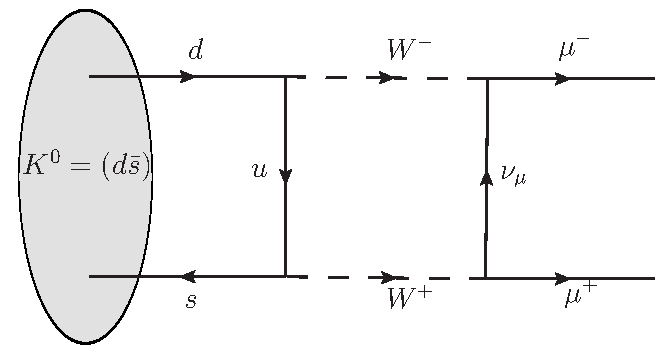
\includegraphics[scale=0.8]{Ktomumu}
\caption{Decaimiento de $K^{0} \to \mu^{+} + \mu^{-}$.}
\label{Fig:Ktomumu}
\end{figure}
%

Para explicar la violación de CP es necesario un número complejo en la matriz de \textquotedblleft rotación\textquotedblright \eqref{Eq:Rot}. Debido a que es posible eliminar las fases complejas de las matrices $2 \times 2$ mediante una redefinición adecuada de las fases de los quarks, no es posible explicar la violación de CP con el mecánismo de GIM. En 1973 antes de que el quark $c$ fuera descubierto, los físicos Japoneses Makoto Kobayashi y Toshihide Maskawa propusieron una explicación a la violación de CP dentro del esquema de Cabibbo-GIM~\cite{Kobayashi:1973fv}. Su propuesta consistía en definir la matriz de rotación $3 \times 3$, generalizando así, la matriz de Cabibbo a la matriz de Cabibbo–Kobayashi–Maskawa (o matriz $V_{\text{CKM}}$). Con esto era posible mantener la fase compleja. Además, se daba cuenta de la existencia de una tercera generación de quarks, conocidas como \textquotedblleft las generaciones de interacción débil\textquotedblright
%
\begin{align*}
\begin{pmatrix}u \\ d' \end{pmatrix}\,, & 
&\begin{pmatrix}c \\ s' \end{pmatrix}\,, &
&\begin{pmatrix}t \\ b' \end{pmatrix}\,,
\end{align*}
%
las cuales están relacionadas con  los estados de quarks físicos mediante la matriz $V_{\text{CKM}}$
%
\begin{align*}
\begin{pmatrix}d' \\ s' \\ b' \end{pmatrix} =& 
\begin{pmatrix}V_{ud} & V_{us} & V_{ub} \\ V_{cd} & V_{cs} & V_{cb} \\ V_{td} & V_{ts} & V_{tb} \end{pmatrix}
\begin{pmatrix}d \\ s \\ b \end{pmatrix}
\end{align*}
%
donde $V_{q q'}$ hace referencia a las mezclas entre el quark $q$ y el $q'$. Por ejemplor, $V_{ud}$ hace referencia a la mezcla $u + \bar{d} \to W^{-}$. Por lo que hay nueve entradas en la matriz $V_{\text{CKM}}$, pero no todos son parámetros independientes, ya que es posible llevar esta matriz a su forma canonica, en esta forma dicha matriz dependerá de los ángulos de Cabibbo generalizados ($\theta_{12}$, $\theta_{13}$ y $\theta_{23}$) y una fase $\delta$
%
\begin{align*}
V_\text{CKM} =& 
\begin{pmatrix}
c_{12} c_{13} & s_{12} c_{13} & s_{13} e^{-i\delta} \\ 
-s_{12} c_{23} - c_{12} s_{23} s_{13} e^{i\delta} & c_{12} c_{23} - s_{12} s_{23} s_{13} e^{i\delta} & s_{23} c_{13} \\ 
s_{12} s_{23} - c_{12} c_{23} s_{13} e^{i\delta} & -c_{12} s_{23} - s_{12} c_{23} s_{13} e^{i\delta} & c_{23} c_{13} 
\end{pmatrix}\,,
\end{align*}
%
donde $c_{ij} = \cos \theta_{ij}$ y $s_{ij} = \sin \theta_{ij}$. Si hacemos $\theta_{23} = \theta_{13} = \delta = 0$ y $\theta_{12} = \theta_C$, la tercera generación no se mezcla con las otras dos y es posible recuperar la teoría de  Cabibbo-GIM. Sin embargo, debido al decaimiento del mesón $B^{-}$($\bar{u}b$) se sabe que la tercera familia se mezcla a la primera, aunque esta mezcla debe ser bastante pequeña para poder explicar el éxito del esquema Cabibbo-GIM original. Además, debido a que el ME no ofrece ninguna predicción sobre los valores de la matriz  $V_{\text{CKM}}$ solo se conocen los valores de los elementos de la matriz mediante los diferentes  experimentos diseñados para medir éstos. Las magnitudes y su precisión están dados por:
%
\begin{align*}
V_{\text{CKM}} =& 
\begin{pmatrix}
0.97427\pm 0.00015 & 0.22534\pm 0.00065 & 0.00351^{+0.00015}_{-0.00014} \\ 
0.22520\pm 0.00065 & 0.97344\pm 0.00016 & 0.0412^{+0.0011}_{-0.0005} \\ 
0.00867^{+0.00029}_{-0.00031} & 0.0404^{+0.0011}_{-0.0005} & 0.999146^{+0.000021}_{-0.000046}
\end{pmatrix}\,,
\end{align*}
%
y la fase tiene un valor de $\delta = 1.20 \pm 0.08$. La mezcla de la tercera familia (los elementos  de la tercera fila y columna fuera de la diagonal) con las demás resulta ser muy pequeña, debido a la larga vida del mesón $B$ ($10^{-12}$ seg)~\cite{Beringer:1900zz}.


\section{Universalidad}

En el ME de partículas, cada fermión tiene tres copias idénticas, siendo la masa la única diferencia entre ellas. A cada una de dichas copias se les conoce como familias o generaciones de fermiones. Debido a esto no es posible diferenciar entre una familia u otra en procesos físicos en los que masa no sea un parámetro relevante. Esta propiedad emergente del ME se conoce como universalidad.

Para comprobar la universalidad del bosón $W$ es necesario determinar los anchos de decaimiento, por lo que es necesario conocer el lagrangiano de interacción. El Lagrangiano que describe la interacción de los fermiones al bosón $W$ es:
%
\begin{align}\label{Eq:LagW}
\mathcal{L} = \frac{g_W}{\sqrt{2}} (\overline{q'} {W}_{\mu}^{-}  \gamma ^{\mu} V_{\text{CKM}} P_{L} q + \overline{\nu_{\ell}} {W}_{\mu}^{-} \gamma ^{\mu} P_{L} \ell^{-}) + \text{h.c.}\,,
\end{align}
%
donde $P_{L} = (1 - \gamma_5)/2$ es el proyector izquierdo, $q$ y $q'$ hacen referencia a los quarks ($u$, $d$, $c$, $s$, $b$ y $t$), $\ell$ hace referencia a los diferentes leptones ($e$,$\mu$ y $\tau$).

Debido a que el quark $t$ es más pesado que el bosón $W$, los decaimientos $W \to t d$, $W \to t s$ y $W \to t b$ no son permitidos, por lo que el ancho total de decaimiento del $W$ sería dividido en dos partes, las cuales dependen del producto de estados finales
%
\begin{align}\label{Eq:AnchoW}
\Gamma_{tot} (W) = \sum_{q q^{\prime}}\Gamma(W \to q \bar{q}^{\prime}) + \sum_{\ell} \Gamma(W \to \ell \bar{\nu_{\ell}})\,,
\end{align}
%
donde $q = u$, $c$, $q' = d$, $s$, $b$ y $\ell = e$, $\mu$, $\tau$. Para efectos prácticos se considera que todos los quarks son no masivos excepto el quark $t$, ya que la masa del $W$ es mucho mayor que la masa de los demás quarks. Los anchos de decaimiento para los miembros derechos de la ecuación \eqref{Eq:AnchoW} están dados por:
%
\begin{align}\label{Eq:Gamma}
\Gamma(W \to q \bar{q'}) =& \frac{|V_{\text{CKM}qq'}|^2 g_W^2}{16 \pi} M_{W} \approx 0.6757 |V_{\text{CKM}qq'}|^2 \text{ GeV}\,, \\
\Gamma(W \to \ell \bar{\nu_{\ell}}) =& \frac{g_W^2}{48 \pi} M_{W}\approx 0.2252 \text{ GeV}\,,
\end{align}
%
donde $g_W^2 = 8M^2_{W}G_F / \sqrt{2}$ y $V_{\text{CKM}qq'}$ son las respectivas entradas de la matriz $V_{\text{CKM}}$, $M_{W}$ es la masa del bosón $W$ y $G_F$ es la constante de Fermi. El ancho total de decaimiento para el bosón $W$ es:
%
\begin{align}
\Gamma_{tot}(W) =& \frac{g_W^2}{16 \pi}\left[\sum_{q q^{\prime}} |V_{\text{CKM}qq'}|^2 + 1 \right] M_{W}\,.
\end{align}
%
Haciendo la suma sobre la CKM, tenemos \begin{align*}
\sum_{q q^{\prime}} |V_{\text{CKM}qq'}|^2 = 1.99999 \approx 2.0 \,,
\end{align*} por lo que la amplitud total de decaimiento toma la forma:
%
\begin{align}
\Gamma_{tot}(W) =& \frac{3 g_W^2}{16 \pi} M_{W} \approx 2.094 \text{GeV}\,,
\end{align}
%
y los branching son iguales a
%
\begin{align}\label{Eq:Branching}
B(W \to \ell \nu_{\ell}) =& \frac{1}{9} \approx 11.1\% \,, & 
B(W \to \text{Hadrones})= \sum_{q q^{\prime}} B(W \to q \bar{q'}) =& \frac{2}{3} \approx 66.6\%\,.
\end{align}
%
Lo cual concuerda con los resultados experimentales~\cite{Beringer:1900zz}
\begin{align*}
B(W \to \ell \nu_{\ell}) =& (10.80 \pm 0.09)\%\,, & B(W \to \text{Hadrones})= \sum_{q q^{\prime}} B(W \to q \bar{q'}) =& (67.60 \pm 0.27)\%\,.
\end{align*} 
%
Debido a que en las desintegraciones débiles de alta energía los efectos de la masa son despreciables en la Eq. \eqref{Eq:Gamma}, el bosón $W$ debe de decaer con igual probabilidad a las diferentes familias de leptones. Esta propiedad emergente se le conoce como la Universalidad Leptónica (UL), la cual implica que los bosones vectoriales se acoplan por igual a las tres familias de leptones. 
En particular, las mediciones de los decaimientos $b \rightarrow c \ell \nu$ para diferentes leptones de estado final, pueden ser utilizadas probar la UL con una gran precisión, dado la cancelación de muchas fuentes de incertidumbres teóricas que ocurren en relaciones, tales como:
\begin{align}
R(D^{(*)}) = \frac{\Gamma(B \rightarrow D^{(*)} \tau \nu)}{\Gamma(B \rightarrow D^{(*)} \ell \nu)}\,,
\end{align}
con $\ell = e$ o $\mu$. El ME predice que los valores para dichos procesos deben ser $R(D) = 0.298 \pm 0.003$ y $R(D^*) = 0.255 \pm 0.004 $. Adicionalmente, las mediciones de la razón
\begin{align}
R_K = \frac{\Gamma(B \rightarrow K \mu ^+ \mu ^-)}{\Gamma(B \rightarrow K e^+ e^-)}\,,
\end{align}
deben respetar la UL y por lo tanto el valor predicho por el ME es $R_K = 1.0$~\cite{Beringer:1900zz}.

\chapter{Bosón $W^{\prime}$}\label{Ch:W-prime}
La gran mayoría de los modelos con Física Más Allá de ME (BSM, por sus siglas en ingles) predicen  partículas adicionales al ME. El interés principal en este trabajo consiste en adicionar un bosón vectorial cargado y pesado, generalmente denotado como $W^{\prime}$, con carga $\pm 1$ y espín $1$. En general, dichos modelos también predicen un bosón vectorial neutral, denotado como $Z^{\prime}$. 

Para generar un nuevo bosón vectorial cargado, algunos modelos adicionan dimensión extras a las cuatro dimensiones conocidas. Debido a que estas dimensiones están compactificadas, no es posible verlas a escalas de bajas energía.  Debido a la compactificación de dichas dimensiones, se crean los llamados modos de Kaluza-Klein, que son excitaciones de las partículas del ME en las dimensiones extra. Esto puede predecir excitaciones del  bosón $W$, generando un $W^{\prime}$~\cite{Chen:2009gz, Kong:2010xk}.

Otros modelos proponen una simetría izquierda-derecha, adicionando al grupo mediador del ME un grupo $SU (2)_R$. Después del rompimiento espontaneo de la simetría de este grupo se generan bosones gauge adicionales, tales como, un bosón $W^{\prime}$ y un bosón $Z^{\prime}$~\cite{Boucenna:2016wpr}. Un modelo de referencia que proporciona un $W^{\prime}$ genérico, es el Modelo Estándar Secuencial (MES)~\cite{Altarelli:1989ff}, el cual supone que existe una copia de los bosones $W$ y $Z$ del ME, con masas más grandes ($Z^{\prime}$ y $W^{\prime}$). Los acoples de estos nuevos bosones son diferentes a los bosones del ME.

El Lagrangiano invariante de Lorentz más general posible que describe el acoplamiento de un $W^{\prime}$ a los fermiones del ME, se puede escribir como:
\begin{align}\label{Eq:Lag}
\mathcal{L} = \frac{g}{\sqrt{2}} (Y^{L}_{f_i f^{\prime}_j} W^{\prime}_{\mu} \bar{f}^{i} \gamma^{\mu} P_L f^{j} + Y^{R}_{f_i f^{\prime}_j} W^{\prime}_{\mu} \bar{f}^{i} \gamma^{\mu} P_R f^{j} ) + \text{h.c.}\,,
\end{align}
donde $P_{R,L} = (1 \pm \gamma_5)/2$ es el proyector derecho e izquierdo respectivamente, $g$ es la constante de acople de $SU(2)_L$ del ME, y las $Y^{R,L}_{f_i f^{\prime}_j}$ son los acoples, los cuales son diferentes para cada fermión, ya sea quark o leptón. Para el caso del bosón $W$ del ME, debido a que este solo se acopla a las corrientes izquierdas, tenemos $Y^{R} = 0$, y $Y^{L}$ serían matrices identidad o las respectivas matrices de Cabibbo-Kobayashi-Maskawa (CKM), para leptones y quarks, respectivamente.

Debido a que los acoples del $W^{\prime}$ pueden ser diferentes a los acoples del $W$ del ME, el branching y el ancho de decaimiento  pueden modificarse con respecto al valor del ME. Además, si el $W^{\prime}$ es más pesado que el quark top y el bottom, el decaimiento $W^{\prime} \to t b$ es permitido. Igualmente, los decaimientos de $WZ$ deberían ser tomados en cuenta, pero debido a que estos dependen del modelo, se asume que estos acoples están suprimidos. El ancho total de decaimiento del $W^{\prime}$ sería dividido en tres partes, las cuales dependen del producto de estados finales
%
\begin{align}\label{Eq:Ancho}
\Gamma_{tot} (W^{\prime}) = \sum_{q} \Gamma(W^{\prime} \to t \bar{q}) + \sum_{q q^{\prime}}\Gamma(W^{\prime} \to q \bar{q}^{\prime}) + \sum_{\ell} \Gamma(W^{\prime} \to \ell \bar{\nu_{\ell}})\,,
\end{align}
%
donde $q = u, d, c, s, b$, $\ell = e, \mu, \tau$. Ya que para efectos prácticos el único quark que se considera masivo es el top, por lo que su masa tendrá una contribución en el ancho de decaimiento del $W^{\prime}$. Los anchos de decaimiento para los miembros derechos de la ecuación \eqref{Eq:Ancho} están dados por:
%
\begin{align}
\Gamma(W^{\prime} \to t \bar{q}) =& \frac{|Y_{tq}|^2 g^2}{16 \pi} M_{W^{\prime}}\left( 1 - \frac{M_{t}^2}{M_{W^{\prime}}^2} \right)\left( 1 + \frac{M_{t}^2}{2M_{W^{\prime}}^2} \right)\,, \\
\Gamma(W^{\prime} \to q \bar{q}^{\prime}) =& \frac{|Y_{q q^{\prime}}|^2 g^2}{16 \pi} M_{W^{\prime}}\,, \\
\Gamma(W^{\prime} \to \ell_L \bar{\nu}_{\ell}) =& \frac{|Y_{\ell \bar{\nu}_{\ell}}|^2 g^2}{48 \pi} M_{W^{\prime}}\,,
\end{align}
%
donde $M_{t}$ es la masa del quark top, y se asume que $g^2 = 8M_{W}G_F / \sqrt{2}$ como en el ME. Es de anotar que los anchos de decaimiento del $W^{\prime}$ tienen la misma forma que los del $W$ de ME. La diferencia en los decaimientos está en que $V_{q q^{\prime}}$ se ha reemplazado por $Y_{q q^{\prime}}$, donde $V_{q q^{\prime}}$ son las entradas de la matriz $V_{\text{CKM}}$. El ancho total de decaimiento para el bosón $W^{\prime}$ es:
%
\begin{align}
\Gamma_{\text{tot}}(W^{\prime}) =& \frac{g^2}{16 \pi}\left[\sum_{q}|Y_{tq}|^2 \left( 1 - \frac{M_{t}^2}{M_{W^{\prime}}^2} \right)\left( 1 + \frac{M_{t}^2}{2M_{W^{\prime}}^2} \right) + \sum_{q q^{\prime}} |Y_{q q^{\prime}}|^2 + \sum_{\ell} \frac{|Y_{\ell \bar{\nu}_{\ell}}|^2}{3}\right] M_{W^{\prime}}\,.
\end{align}
%
Comparando con el ancho de decaimiento del bosón $W$ del ME, se tiene una relación entre estos que está dado por la siguiente ecuación:
%
\begin{align*}
\frac{\Gamma_{\text{tot}}(W^{\prime})}{\Gamma_{\text{tot}}(W)}  =& \frac{4}{3} \frac{M_{W^{\prime}}}{M_{W}}\left[\sum_{q}|Y_{tq}|^2 \left( 1 - \frac{M_{t}^2}{M_{W^{\prime}}^2} \right)\left( 1 + \frac{M_{t}^2}{2M_{W^{\prime}}^2} \right) + \sum_{q q^{\prime}}|Y_{q q^{\prime}}|^2 + \sum_{\ell} \frac{|Y_{\ell \bar{\nu}_{\ell}}|^2}{3}\right]\,.
\end{align*}
%
Si se asume que $M_{W^{\prime}} \gg M_{t}$, el branching adquiere la siguiente forma:
%
\begin{align}\label{Eq:Branching}
B(W^{\prime} \to \bar{f} f^{\prime}) = \frac{C_{f f^{\prime}}|Y_{f f^{\prime}}|^2}{ \sum_{f_1 f_1^{\prime}} C_{f_1 f_1^{\prime}} |Y_{f_1 f_1^{\prime}}|^2 }\,,
\end{align}
%
donde $C_{f f^{\prime}}$ hace referencia al factor de color de los fermiones, el cual es $1$ para leptones y $3$ para quarks. 

\section{No niversalidad del $W^{\prime}$}\label{Sec:NoUL}

La Universalidad Leptónica(UL) en el ME se debe a que las tres familias poseen igual hipercarga débil. Además, ésta podría surgir accidentalmente en el ME a bajas energías; lo que implicaría que las anomalías de la universalidad leptónica observadas podrían deberse a que el ME sería un modelo efectivo hasta la escala de TeV.

Sin embargo, no es necesario abandonar la idea de UL para el bosón $W$, debido a que es posible dar explicación a las anomalías observadas, considerando que estas están asociadas con física BSM. Se han propuesto varios modelos teóricos que dan explicación a las anomalías. Dado que, tanto las corrientes débiles neutras, como las corrientes débiles cargadas presentan dichas anomalías, un modelo que da explicación a éstas es el de leptoquarks (LQ)~\cite{Sakaki:2013bfa}. 

Otros modelos que dan explicación a estas anomalías son conocidos como modelos no universales. En estos modelos, se adicionan bosones gauge que se acoplan de forma distinta a las familias de quarks y leptones. La explicación más natural para las anomalías asociadas a corrientes débiles neutras, es la existencia de un nuevo bosón débil neutro, llamado Z prima ($Z^{\prime}$), el cual se acopla de forma diferente a las familias de leptones. Este nuevo bośon puede ser generado a partir de adicionar una  nueva simetría $U(1)$ al ME~\cite{Dalchenko:2017shg}. Ahora, la explicación más natural para las anomalías asociadas a corrientes débiles cargadas, es la existencia de nuevos bosones débiles cargados, llamados $W^{\pm}$ primas ($W^{\prime \pm}$), los cuales se acoplan de forma diferente a las familias de leptones y quarks. Estos nuevos bosones pueden ser generados a partir de adicionar una nueva simetría no Abeliana $SU(2)$ al ME. Es de notar, que es posible incorporar la primera solución a la segunda, en analogía con la simetría $SU(2)$ electrodébil del ME~\cite{Boucenna:2016wpr} donde coexisten el $W$ y el $Z$. 
En dicho modelo también se muestra un mecanismos que permite caracterizar la no universalidad del bosón $W^{\prime}$. Como resultado se obtiene que el $W^{\prime}$ no se acopla a la primera familia. Además, la interacción con la segunda y tercera generación es diferente en general.

Debido a que el interes de este trabajo es poder dar una explicación a las anomalías en $R(D^{(*)})$, tenemos que el decaimiento del mesón $B$ en el ME va a estar suprimido por la $V_{cb}$ de la CKM, como se muestra en la fig.~\ref{Fig:BW_decay}. Por lo tanto es necesario introducir una nueva contribución de las corrientes cargadas, para poder dar explicación a las anomalías. Esta nueva corriente carga se genera apartir de un $W^{\prime}$ no universal.  Las contribuciones debidas al $W^{\prime}$ en $R(D^{(*)})$ se genera por el decaimiento del quark $b$ a un quark $c$ y un bosón $W^{\prime}$, donde a la vez, el $W^{\prime}$ decae a un $\tau$ y a un $\nu$(ver fig.~\ref{Fig:BWp_decay}). Una explicación más detallada de éste modelo se da en el siguiente capítulo.

%
\begin{figure}
\centering
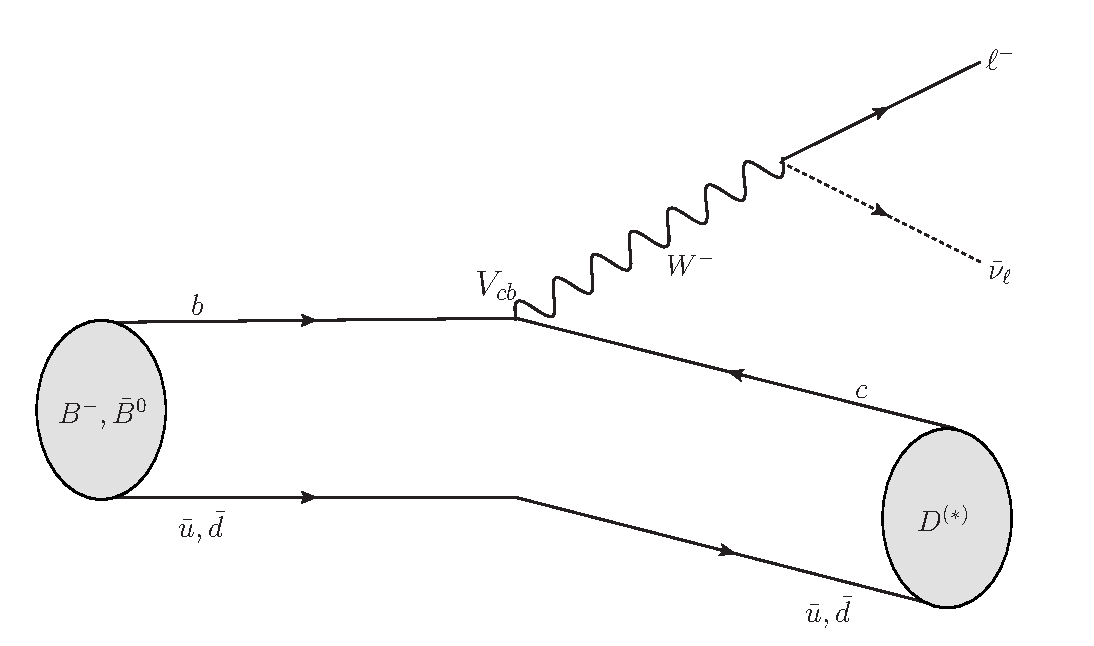
\includegraphics[scale=0.6]{figures/BW_decay}
\caption{Decaimiento en el ME de los mesones $B^{-}, \bar{B}^{0} \to D^{(*)} + \ell^{-} + \bar{\nu}_{\ell}$.}
\label{Fig:BW_decay}
\end{figure}
%

%
\begin{figure}
\centering
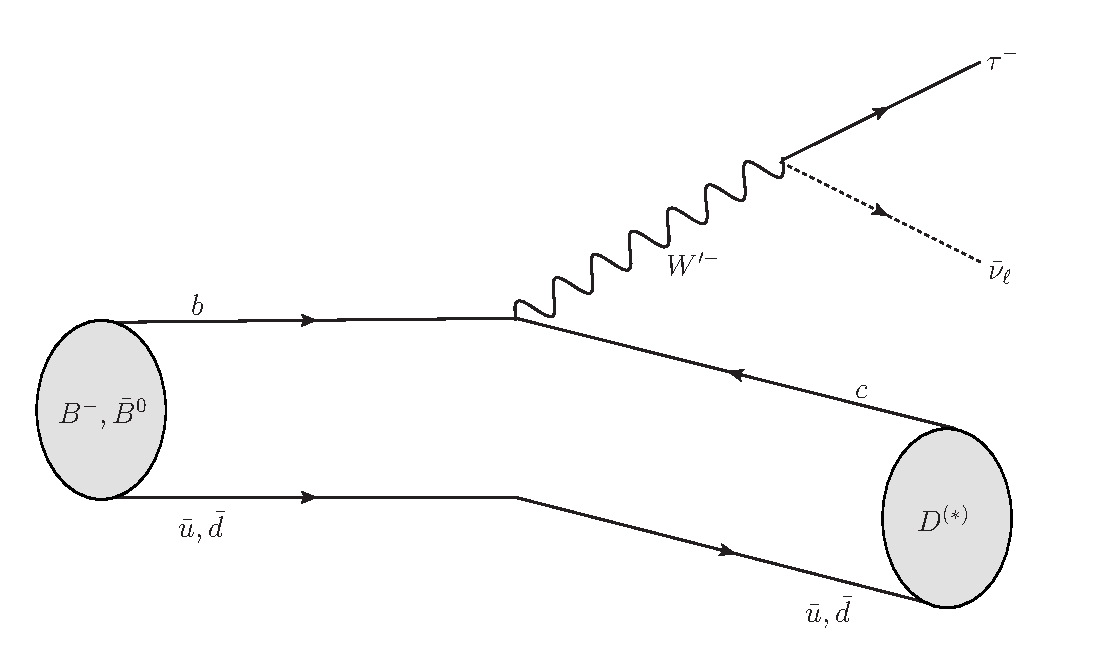
\includegraphics[scale=0.6]{figures/BWp_decay}
\caption{Contribución del $W^{\prime}$ al decaimiento de los mesones $B^{-}, \bar{B}^{0} \to D^{(*)} + \tau^{-} + \bar{\nu}_{\ell}$.}
\label{Fig:BWp_decay}
\end{figure}
%
\chapter{$W'$ y las anomalías en $R(D^{(*)})$}
\label{Ch:results}
Debido a que el decaimiento $b \to c \tau \nu$ está suprimido en el ME debido a la CKM(ver fig.~\ref{Fig:BW_decay}), es necesario obtener una nueva contribución a las corrientes cargadas para dar explicación a las anomalías en la medición de $R(D^{(*)})$. Una forma símple es extender el sector escalar del ME con un bosón gauge cargado $W^{\prime}$, el cual sólo se acopla a los fermiones de segunda y tercera generación, haciendo que sea más difícil la detección de este en el LHC. Además, la existencia de $\tau$’s en el estado final conduce a una dificultad, debido al background del ME en el LHC.

Debido a estas condiciones y el interés de esta investigación~\cite{Abdullah:2018ets} se propone que el $W'$ solo se acople a los quarks bottom ($b$) y charm ($c$) en el sector del color y a la tercera familia (sabor $\tau$) en el sector de leptones(ver fig.~\ref{Fig:BWp_decay}). Debido a que la probabilidad de encontrar un $b$ dentro del protón es muy baja, los canales de producción dominantes en este caso son la fusión $g g$ y $g c$, los cuales conducen a un jet $b$ asociado en el estado final. La presencia de este jet $b$ en el estado final da la posibilidad de diferenciar las señales del $W^{\prime}$ respecto al background del ME. Para esto se realiza un análisis exclusivo que requiere al menos un jet $b$ en estado final junto con un $\tau$ hadrónico y energía faltante, mejorando potencialmente la eficiencia de producción. Además, la existencia de un jet $b$ en estado final permitiría deducir la existencia de un acoplamiento a la tercera generación del $W^{\prime}$, lo cual es crucial para la explicación de las anomalías. 

Para comprender mejor la efectividad de esta técnica, contrastemos el uso del b-tags con reinterpretaciones de análisis inclusivos del $W^{\prime}$ realizados por ATLAS y CMS en los que no se hacen tales requisitos de jet $b$. En las Refs.~\cite{Khachatryan:2015pua, Aaboud:2018vgh}, la búsqueda inclusiva de $W^{\prime}$ se realiza sin referencia al mecanismo de producción y, por lo tanto, sin la necesidad del jet $b$. La Ref.~\cite{Altmannshofer:2017poe} considera el proceso $gc \to b \tau$ en el LHC, pero solo como un vértice efectivo y buscando decaimientos leptónicos de $\tau$ en lugar de hadrónicos. Sus resultados no son aplicables al rango de masas de interés en este trabajo. En Ref.~\cite{Asadi:2018wea} Se estudia un $W^{\prime}$ aparentemente idéntico al que se muestra aquí y los límites del colisionador se colocan solo de forma indirecta al reutilizar una búsqueda de ATLAS existente de un bosón gauge $Z^{\prime}$. Sus límites, aunque más concretos desde una perspectiva UV, dependen en gran medida del modelo. En Ref.~\cite{Dalchenko:2017shg}, se demuestra la importancia de los jets $b$ en las búsquedas de resonancias pero usando un bosón gauge $Z^{\prime}$ que decae en muones. Hay que destacar que, independientemente de las anomalías en los mesones $B$, las propiedades mencionadas anteriormente son dignas de investigación por si solas, además de servir como una pieza de rompecabezas adicional en el programa de búsqueda de resonancias en el LHC~\cite{Craig:2016rqv}.

Las interacciones que conectan la nueva física en este modelo con el ME están descritas por el siguiente Lagrangiano:
 %
 \begin{align}\label{Eq:LagWp}
 \mathcal{L} = ( g'_q \overline{c}  \gamma ^{\mu} P_{L} b +g'_{\tau} \overline{\nu}_{\tau}  \gamma ^{\mu} P_{L} \tau^{-}){W^{\prime}}_{\mu}^{+} + h.c.\,,
 \end{align}
 %
donde $g^{\prime}_{q}$ y $g^{\prime}_{\tau}$ son los acoples de nueva física. Debido a que estos acoplamientos violan sabor, construir una afinación UV que sea consistente con el ME no es sencillo. Un ejemplo de tal afinación UV se da en~\cite{Boucenna:2016qad} , donde se supone que el $W^{\prime}$ solo se acopla directamente a una generación de fermiones vector-like demasiado pesados para ser observados. Los acoplamientos en Eq.~\eqref{Eq:LagWp} luego se inducen a través de mezclas entre los nuevos fermiones y los fermiones del ME. En cualquier modelo UV de este tipo, se hacen muchas suposiciones adicionales que deben probarse individualmente en comparación con el experimento, y rara vez se puede descartar todo el espacio de posibles modelos. Por lo tanto, en lugar de demostrar la viabilidad de esta instancia particular de tales modelos, adoptamos el enfoque pragmático de referirnos al mecanismo en~\cite{Boucenna:2016wpr} como una prueba de principio y centrarnos en cambio en las implicaciones del colisionador sobre un constructo mínimo.
%
\begin{figure}
\begin{center}
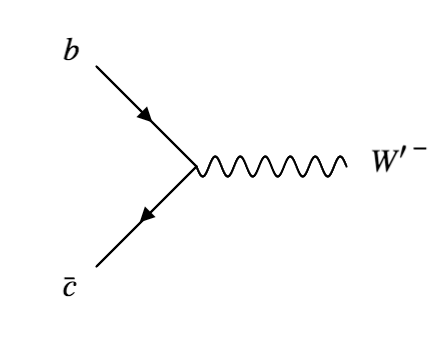
\includegraphics[width = 0.28 \textwidth]{diag_bc.png}
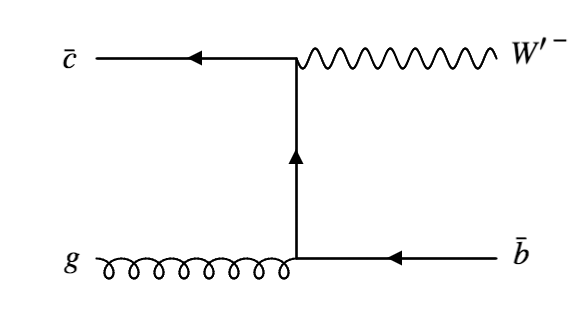
\includegraphics[width = 0.35 \textwidth]{diag_gc.png}
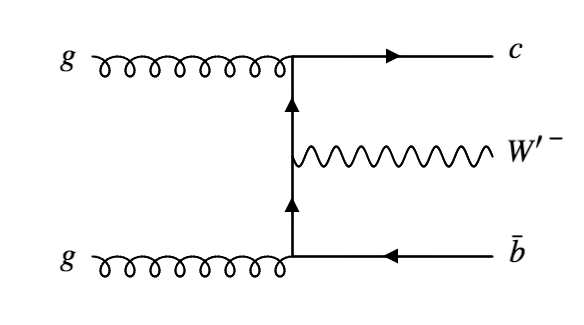
\includegraphics[width = 0.35 \textwidth]{diag_gg.png}
\caption{Representación de diagramas de Feynman de producción de $W'$ en el LHC.}
\label{Fig:diag}
\end{center}
\end{figure}
%

Los principales canales de producción del $W^{\prime}$ en el LHC se muestran en la Fig.~\ref{Fig:diag}. La producción a través de cualquier otro estado inicial se suprime por medio de acoplamientos adicionales. Para acoplamientos y número de estados finales mayores las contribuciones en sección transversal de estos diagramas estarían ordenados de izquierda a derecha. Esto se contrarrestaría con la diferencia en la fracción de momento transportada por gluones, quarks $c$  y quarks $b$. Uno esperaría que los diagramas con gluones en el estado inicial sean dominantes. Como se vera, la eficiencia del requisito del b-tags sugiere que esto es cierto en buena medida.

Debido a que el rango de masas que se toma en cuenta está por encima de los $200$ GeV, todos los productos de los decaimientos son no masivos, lo cual ayuda a simplificar las expresiones para los branchings, los cuales se pueden calcular de la Eq.~\eqref{Eq:Branching}:
%
\begin{align}
B({W'}^+ \to \tau^+\nu_{\tau}) \approx& \frac{|g'_{\tau}|^2}{|g'_{\tau}|^2+3 |g'_q|^2}\,, &
B({W'}^+ \to c\bar{b} ) \approx& \frac{3 |g'_{q}|^2}{|g'_{\tau }|^2+3 |g'_{q}|^2}\,.
\end{align}
%
Siguiendo~\cite{Boucenna:2016qad}, los observables van a estar dados por:
%
\begin{align}
R(D^{(*)})_{\text{NF}} = \left( 1 + \frac{g'_{\tau}g'_q}{m^2_{W'}} \frac{\sqrt{2}}{4 G_F V_{cb}}\right)^2 R(D^{(*)})_{\text{ME}}\,,
\end{align}
%
donde $m_{W'}$ es la masa del bosón $W'$, $G_F = 1.16 \times 10^{-5}$ GeV$^2$ es la constante de Fermi, y $V_{cb} = 0.04$ es la componente $cb$ de la matriz CKM. Definiendo los nuevos acoples positivos, el valor central para $R(D)$ y $R(D^{*})$ requieren que el factor $g'_qg'_{\tau}/m^2_{W'}$ sea igual a $0.002(100\text{ GeV}/m_{W'})^2$ y $0.001(100\text{ GeV}/m_{W'})^2$ respectivamente. En este estudio se presentan límites en el plano $m_{W'}-g'_q$ para diferentes valores de $g'_{\tau}$.

\section{Coordenadas en los detectores}
Cada detector en un acelerador está hecho para cubrir un determinado ángulo solido dependido de lo que se quiera estudiar. Dentro del ángulo sólido elegido de un experimento, ninguna partícula debe escapar de la detección, excepto por los neutrinos, los cuales debido a su interacción débil no interactúan en la escala de longitud de un detector típico. Todas éstas partículas que escapan del detector son conocidas como energía transversa faltante $E^{\text{miss}}_T$.

El sistema de coordenadas en los detectores del LHC se definen de la siguiente manera: 
El punto de interacción se define como el origen del sistema de coordenadas. El eje $z$ corre a lo largo de la línea del haz. El plano $x$ - $y$ es perpendicular a la línea del haz y se conoce como el \textquotedblleft plano transversal\textquotedblright. El eje $x$ positivo apunta desde el punto de interacción al centro del anillo principal del LHC; el eje $y$ positivo apunta hacia arriba de la superficie de la Tierra. En el caso de los detectores cilíndricos, aprovechando su simetría, se utilizan coordenadas cilíndricas. En general el plano transversal se describe en términos de las coordenadas $r$ - $\phi$. El ángulo azimutal $\phi$ se mide desde el eje $x$, alrededor del haz, y el radio $r$, es la longitud desde la línea del haz. El ángulo polar $\theta$ se cuenta desde el eje $z$ positivo. El ángulo polar a menudo también se da en términos de la pseudorapidez, definida como $\eta = -\ln \tan (\theta/2)$.
La pseudo-rapidez es la aproximación sin masa de la variable de rapidez $y$ definida para una partícula con energía $E$, momento $p$ y momento longitudinal $p_L = | p | \sin \theta$ a lo largo del haz como
%
\begin{align*}
y = \frac{1}{2}\ln \frac{E+p_L}{E-p_L} \approx \eta = \frac{1}{2}\ln \frac{|p|+p_L}{|p|-p_L} = -\ln \tan\left( \frac{\theta}{2} \right)\,.
\end{align*}
%
Se usa la pseudorapidez $\eta$ en lugar del ángulo polar porque los detectores son cilindros concéntricos, lo que limita los ángulos polares en los que se obtiene una reconstrucción precisa de la energía transversa $E_T$, de las partículas. Por otra parte, la producción de partículas es aproximandamente, constante en función de $\eta$.

En este sistema de coordenadas en lugar de utilizarse el modulo del momento, se utiliza el momento transverso $p_T$, el cual se define como la componente del momento en el plano transversal $p_T = | p | \cos \theta$. Esta cantidad es importante, ya que es posible calcularla a partir de la $E_T$, depositada en los calorímetros en los detectores.

Señales de nueva física en un colisionador puede ser detectadas mediante el decaimiento del $W^{\prime}$ a un $\tau_h$ y $E^{\text{miss}}_T$. Estas señales pueden ser vistas como una característica en el espectro observado de masa transversal, definido como
%
\begin{align*}
M_{T} = \sqrt{2p^{\tau}_{T} E^{\text{miss}}_{T}(1-\cos [\Delta \phi (p^{\tau}_{T},p^{\text{miss}}_{T})])}\,,
\end{align*}
%
donde $p^{\tau}_{T}$ es la magnitud del vector momento transversal del candidatos a $\tau_h$, $\Delta \phi$ es la diferencia en el ángulo azimutal entre $p^{\tau}_{T}$ y $E^{\text{miss}}_{T}$ y $E^{\text{miss}}_T$ es el modulo de $\vec{p}^{\text{miss}}_{T}$, el cual se define como $-\sum_{i} \vec{p}_{T}$ de todas las partículas que no interaccionan con el detector. Debido a que los decaimientos hadrónicos del lepton $\tau_h$ se pueden diferenciar experimentalmente, debido a su baja multiplicidad de hadrones cargados, a diferencia de los jets que se originan de la hadronización de partones producidos en el proceso de dispersión dura, que tienen alta multiplicidad de hadrones cargados, por lo que $m_{T}$ podría usarse para identificar las resonancías del $W^{\prime}$.

Otra cantidad importante para la reconstrucción de los eventos en el detector es la distancia angular, la cual es definida como $\Delta R = \sqrt{(\Delta \eta)^2+(\Delta \phi)^2 }$.

\section{Muestras y simulaciones}

La producción del par de quarks ($t\bar{t}$) con jets asociados de estados iniciales de radiación (EIR), comunmente referido a un evento semileptónico $t\bar{t}+$jets, donde $t\bar{t} \to b W^+ \bar{b}W^- \to b\bar{b}\ell^{\pm}\nu_{\ell}q\bar{q}$, representa la fuente dominante de background ($61\%$ de el background total). La siguiente fuente de background, 21\%, viene de la producción de un bosón $W$ con jets de EIR ($W+$jets), donde se produce un leptón real de un $W$ y la energía transversal faltante ($E^{\text{miss}}_T$) es obtenida del neutrino asociado del decaimiento del $W$. Los producción de eventos de Drell-Yann (DY) ($Z/\gamma^*$), más un jet de EIR, contribuyen al $11\%$ del background total. El decaimiento leptónico del bosón $Z/\gamma^*$ entrando en los estados finales de los eventos seleccionados cuando uno de los leptones se pierde en la reconstrucción, dando lugar a la energía transversal faltante. Otras contribuciones al background provienen de los eventos con un solo quark top y la producción de pares vectoriales ($WW$, $ZZ$, $WZ$), referidos como un evento dibosónico, más jets de EIR. La señal simulada y el background se calcula a orden principal (LO de las siglas en inglés). Esto fueron producidos usando \textsc{MadGraph} (v.2.6.0)~\cite{Alwall:2014hca} interconectado con \textsc{PYTHIA 8} \cite{Sjostrand:2014zea} para la hadronización de partones y \textsc{DELPHES} (v3.3.2)~\cite{deFavereau:2013fsa} fue usado para incluir la interacción de partículas con el detector (se usaron las tarjetas de configuración de CMS). El modelo fue implementado usando \textsc{FeynRules 2.3}~\cite{Christensen:2008py,Degrande:2011ua,Alloul:2013bka}.

Para los eventos de la señal, los procesos de matching y merging fueron implementados usando el algoritmo MLM~\cite{Alwall:2007fs}. Los parámetros de matching, \textbf{xqcut} y \textbf{qcut} se verificaron para que el resultado de la sección transversal sea razonablemente estable, además posea una transición suave en la taza de distribución diferencial de jets entre los eventos con $N$ y $N + 1$ jets, pero no se optimizaron aún más debido a los problemas inherentes en el modelado de las emisiones de quarks pesados. La variable \textbf{xqcut} define la distancia mínima entre partones en el nivel MadGraph, mientras que la variable \textbf{qcut} establece la dispersión mínima de energía para un jet agrupado en PYTHIA. Para la producción de señal, se usaron \textbf{xqcut} de $30$ y \textbf{qcut} de $60$ donde se uso un valor de 5 para el parámetro \textquotedblleft jet flavor scheme\textquotedblright.

Hay que tener presente que hay una gran incertidumbre sistemática en el proceso de matching que no tenemos en cuenta. Esta incertidumbre es mayor cuando los diagramas de mayor multiplicidad (los dos diagramas de la derecha de la figura~\ref{Fig:diag} se descartan aunque la sección transversal correspondiente no cambie). No esperamos que la incertidumbre afecte la eficiencia de selección de los jets duros que necesitamos, aunque la sección transversal total podría en realidad ser mayor o menor hasta en un $30\%$. Esto modifica la sensibilidad proyectada absoluta, pero la comparación entre el análisis exclusivo e inclusivo sigue siendo válida.

Otra posible fuente de error son las divergencias colineales a altas masas de $W'$ en el segundo y tercer diagrama (Fig.~\ref{Fig:diag}), los cuales pueden arruinar la validez del cálculo perturbativo. Una forma de evitar esto es restringir el valor de corte de $p_T$ del $b$-jet como se prescribe en \cite{Degrande:2016aje}. Alternativamente, podemos simular los eventos en NLO con una cascada de partones adecuada para extender el dominio de validez de nuestro corte de $p_T$. Siguiendo el procedimiento utilizado por \cite{Fuks:2017vtl} generamos archivos del modelo compatibles con los cálculos de NLO utilizando \textsc{FeynRules 2.3} \cite{Degrande:2014vpa} y producimos muestras para compararlas con los resultados LO. Encontramos que la sección transversal aumenta aproximadamente un 15\% para una masa del $W'$ de 200 GeV y aproximadamente un 7\% para una masa del $W'$ de 1 TeV para NLO en comparación con LO, mientras que cualquier alteración en la distribución $b$-jet $p_T$ es insignificante (ver apéndice \ref{LOvsNLO}). Usamos los resultados LO para establecer nuestra sensibilidad teniendo en cuenta que los resultados de NLO mejorarían nuestro alcance.

Las simulaciones son afectadas por las incertidumbres asociadas con la generación de los eventos, la simulación del detector y la determinación de la luminosidad integrada. La incertidumbre en la luminosidad integrada es de $2.6\%$~\cite{CMS-PAS-LUM-13-001}. La incertidumbre en la escala de energía del $\tau$ es del $3\%$ para eventos con bajo $p_{T}$~\cite{Khachatryan:2015dfa}. La escala de energía de los jets tiene una incertidumbre entre $3\%$ y $5\%$, dependiendo del $p_{T}$ y el $\eta$~\cite{Khachatryan:2016kdb}. La probabilidad de clasificar un electrón como un $\tau_h$  es de $3-14\%$~\cite{ATLAS-CONF-2017-029}. La incertidumbre en $E^{\text{miss}}_{T}$ es despreciable para $E^{\text{miss}}_{T} > 300$ GeV y del $10\%$ aproximadamente para $E^{\text{miss}}_{T} < 300$ GeV~\cite{Aaboud:2018vgh}.

Gran parte de las mediciones que se realizan en los experimentos de física de altas energías se definen como ejercicios de conteo (determinar cuantos son los eventos de un proceso especifico), por lo que se describen con la estadística de Poisson. La estadística de Poisson se define como al probabilidad de que ocurran una cantidad determinando de eventos en un cierto periodo de tiempo. Ésta estadística se especializa en la ocurrencia de sucesos de baja probabilidad, lo que la hace optima para describir los eventos de señal ($W^{\prime}$) en comparación con los eventos de background (SM). En una distribución de Poisson, la varianza es igual a $N$, por lo tanto, la desviación estándar es $\sigma = \sqrt{N}$.

Para los datos simulados, podemos encontrar eventos de señal ($S$) y eventos de background (B), por lo que el número total de eventos estará dado por $N = S + B$. La significancía es la probabilidad de que al realizar un experimento, éste rechace la hipótesis incial (ME) , dado que era cierta. Por lo que se puede definir la significancia de la señal como el tamaño de la señal en relación con el error del total de los eventos ($\sigma$), es decir, $S/\sqrt{S+B}$. Esto permite dar cuenta del error de todos los eventos, a diferencia de la definición  de significancia $S/ \sqrt{B}$, la cual solo toma en cuenta el background, por lo que podría sobre estimar la significancia de la señal~\cite{Punzi:2003bu}

\textbf{Nota:} Los archivos del modelo en \textsc{FeynRules}, las \textquotedblleft process cards\textquotedblright para \textsc{MadGraph}, y el notebook de \textsc{Mathematica} usados para este estudio se pueden encontrar en~\cite{mo_abdullah_2018_1240452}. Para propositos de reproducibilidad, utilidad y revisión de pares. Igualmente, los resultados fueron publicados en arXiv:1805.01869 [hep-ph]~\cite{Abdullah:2018ets}

\section{Análisis}\label{sec:Analysis}
%
\vspace{10 pt}
\begin{table}
\begin{center}
\begin{tabular}{ l  c}\hline\hline
Criterio & Selección\\
 \hline
    $N_{\tau_{h}}$       & $\ge$ 1 \\
    $|\eta_{\tau_{h}}|$ & $< 2.3$ \\
    $p_{T} (\tau_{h})$ & $> 80$ GeV \\
    Veto second $\tau_{h}$ &  $> 50$ GeV \& $|\eta_{\tau_{h}}| < 2.3$ \\
    $N_{e/\mu}$ with $p_{T} > 15$ GeV & $= 0$ \\
    $N_{b-\text{jets}}$ & $= 1$\\
    $p_{T} (b-\text{jets})$ & $> 20$ GeV \\
    $|\eta_{b-\text{jets}}|$ & $< 2.5$ \\
    $ E^{\text{miss}}_{T}$ & $> 140$ GeV \\
     $|\Delta \phi (\tau_{h}, E^{\text{miss}}_{T})|$ & $ > 2.4$ \\
   \hline\hline
 \end{tabular}
 \caption {Criterios de selección de eventos usados para el análisis.}
 \label{tab:selections}
\end{center}
\end{table}
%

El decaimiento hadronico del $\tau$ está compuesto de un neutrino y un conjunto de hadrones cargados (típicamente uno o tres piones cargados y hasta dos piones neutros)~\cite{Aad:2014rga}. Lo cual permite diferenciar los $\tau_h$ de los diferentes jet en el proceso. Ya que el análisis requiere al menos un $\tau$ hadrónico de estado final, para identificar un jet como uno $\tau_h$, este debe tener un $p_T > 80$ GeV y $|\eta_{\tau_h}| < 2.3$ para que estén dentro de la región de aceptación del tracker. Eventos con un candidato $\tau_h$ adicional con $p_T > 50$ GeV y $|\eta_{\tau_h}| < 2.3$ fueron prohibidos, lo cual ayuda a reducir las contribuciones de dibosón y DY+jets. Además, en esta parte del espacio de parámetros la eficiencia de identificación y la tasa de identificación de fallas son aceptables~\cite{Padeken:2265826}. 

De las topologías en la fig.~\ref{Fig:diag}, se establece que un jet con $p_T > 20$ GeV y $|\eta_{\tau_h}| < 2.5$ identificados como un quark $b$ sea seleccionado. Ya que al subir el $p_T$ del jet por encima de 20 GeV trae una mejora en la resolución,  por lo que dicho valor se establece como el mínimo $p_T$ para seleccionar un jet~\cite{ATL-PHYS-PUB-2015-023}. 
%
\begin{figure}
\begin{center}
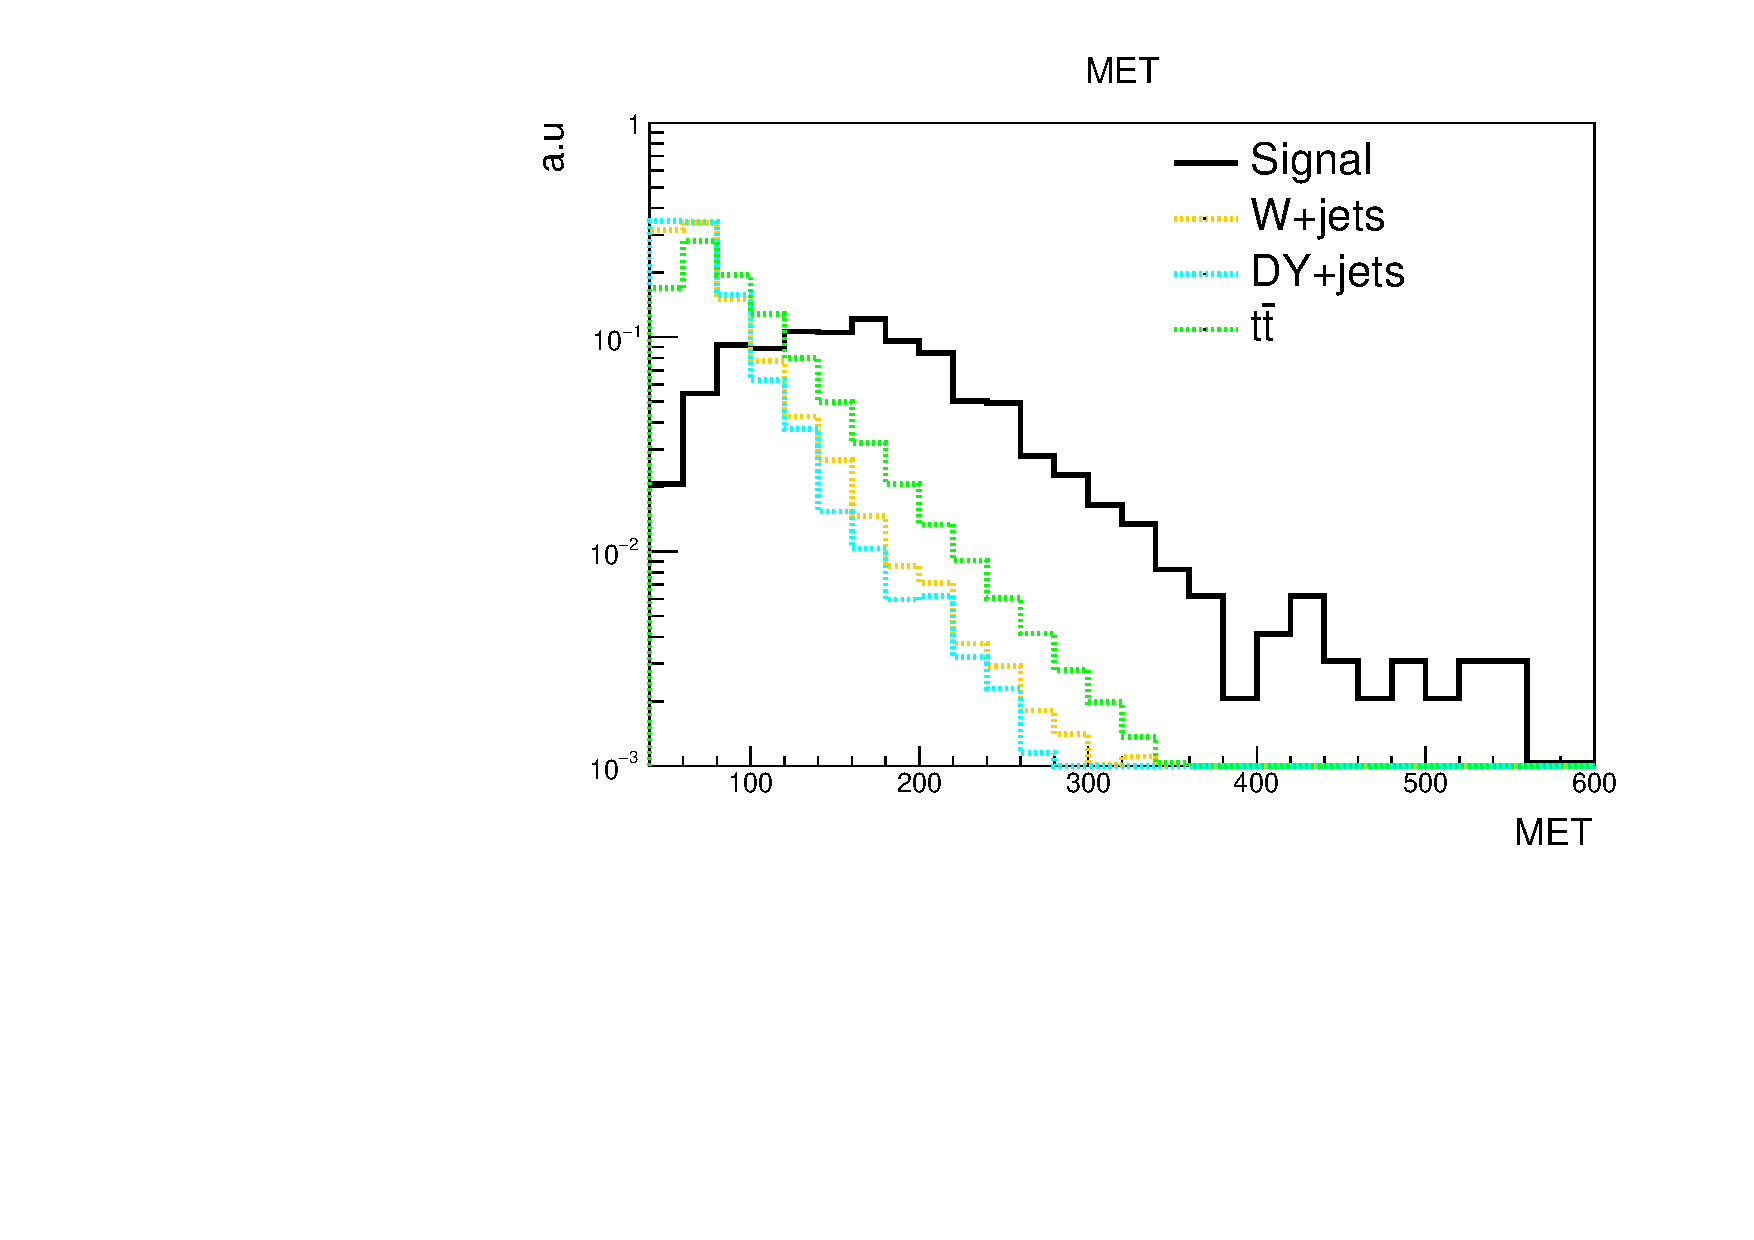
\includegraphics[width = 0.45 \textwidth]{figures/Wp_MET}
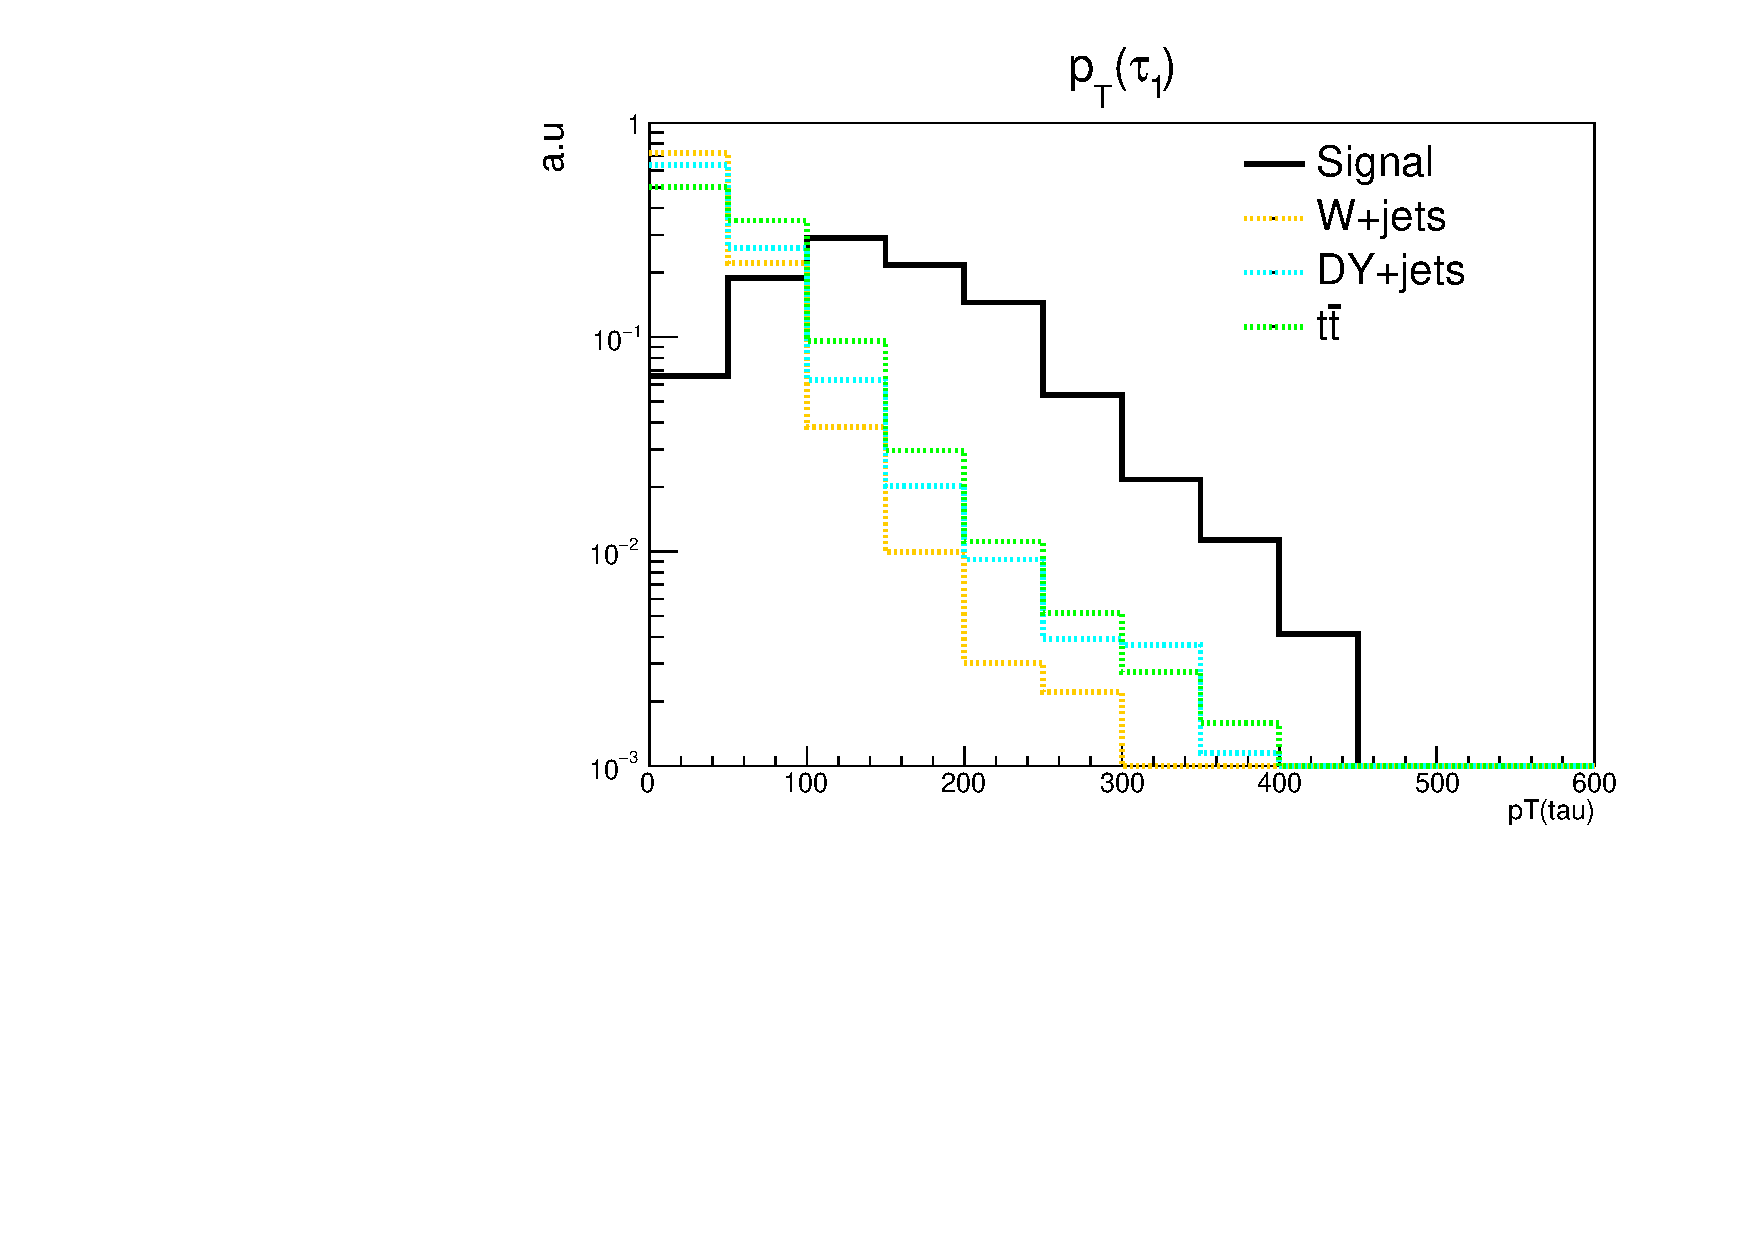
\includegraphics[width = 0.45 \textwidth]{figures/Wp_Tau_pT}
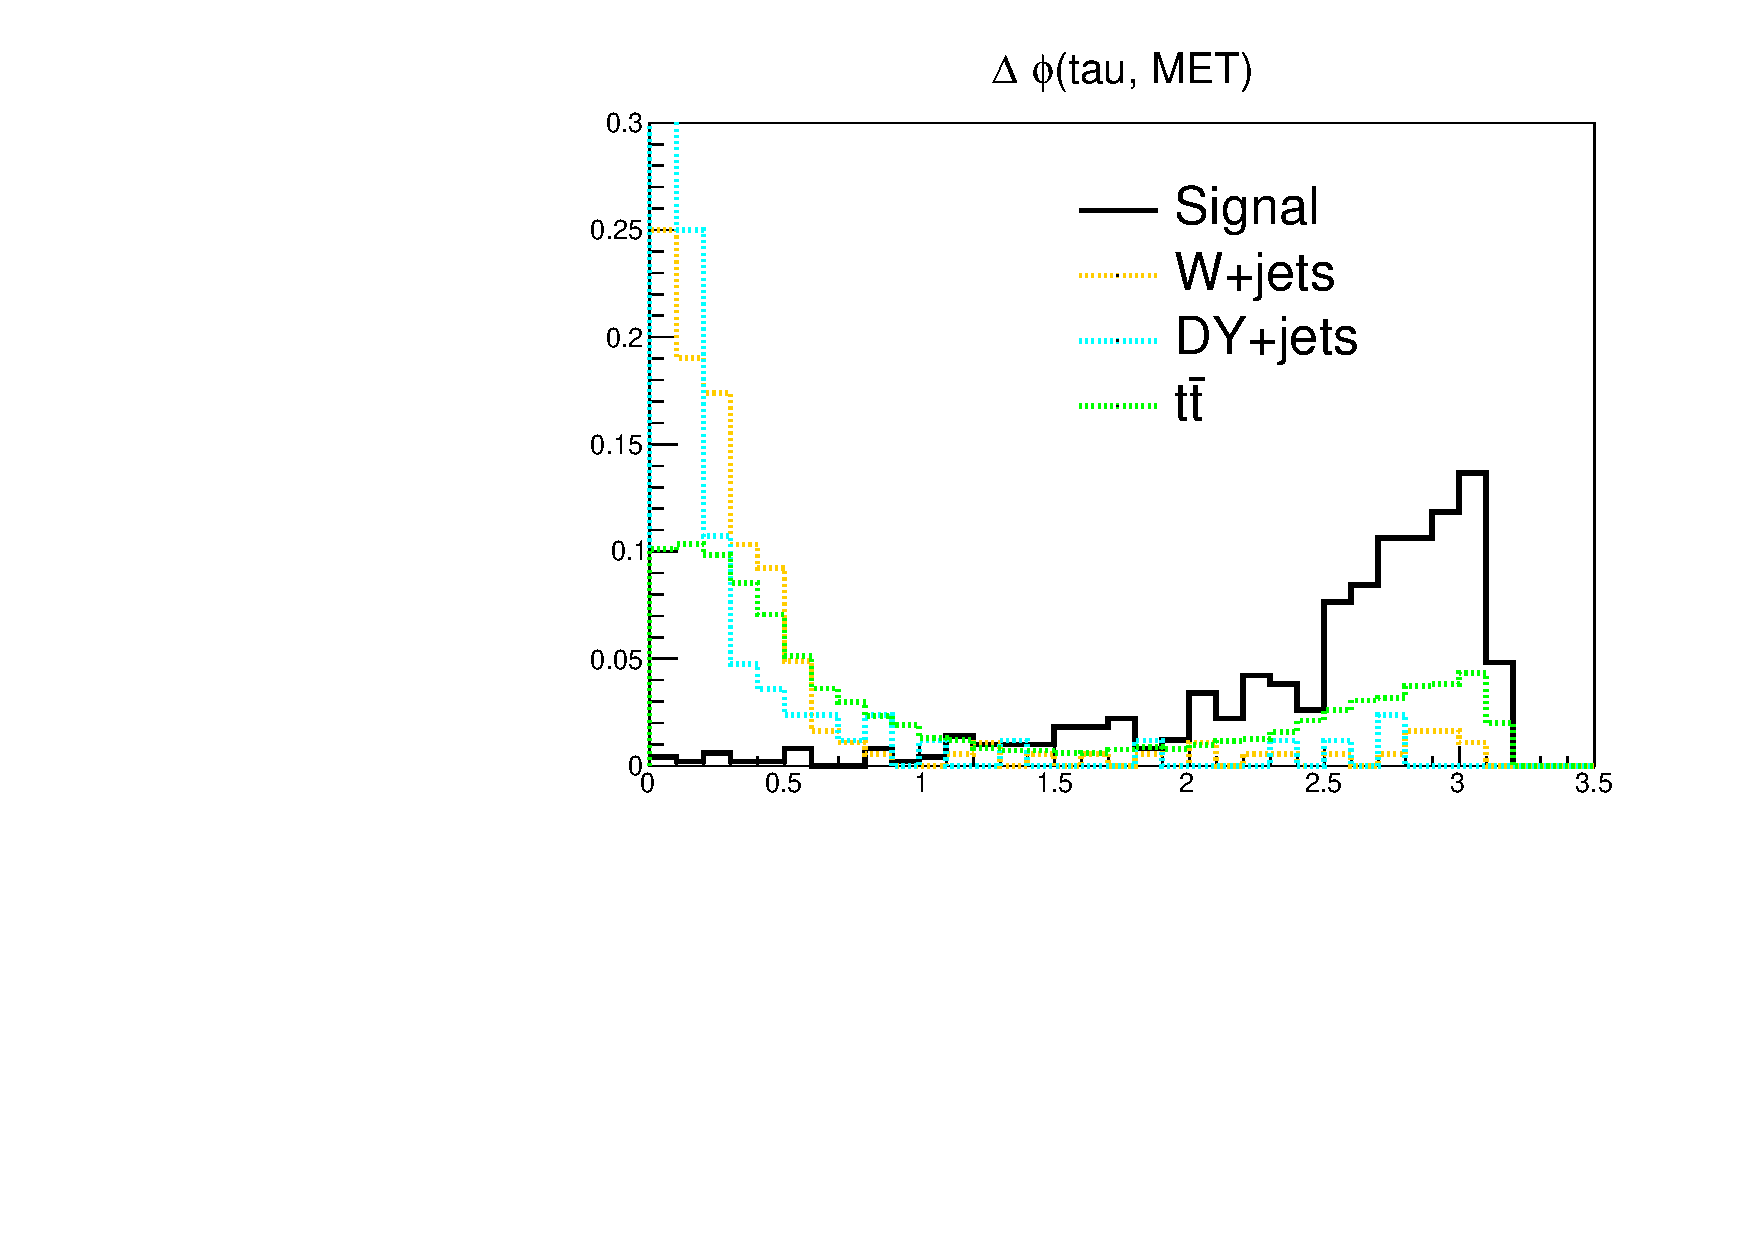
\includegraphics[width = 0.45 \textwidth]{figures/Wp_Delta_phi}
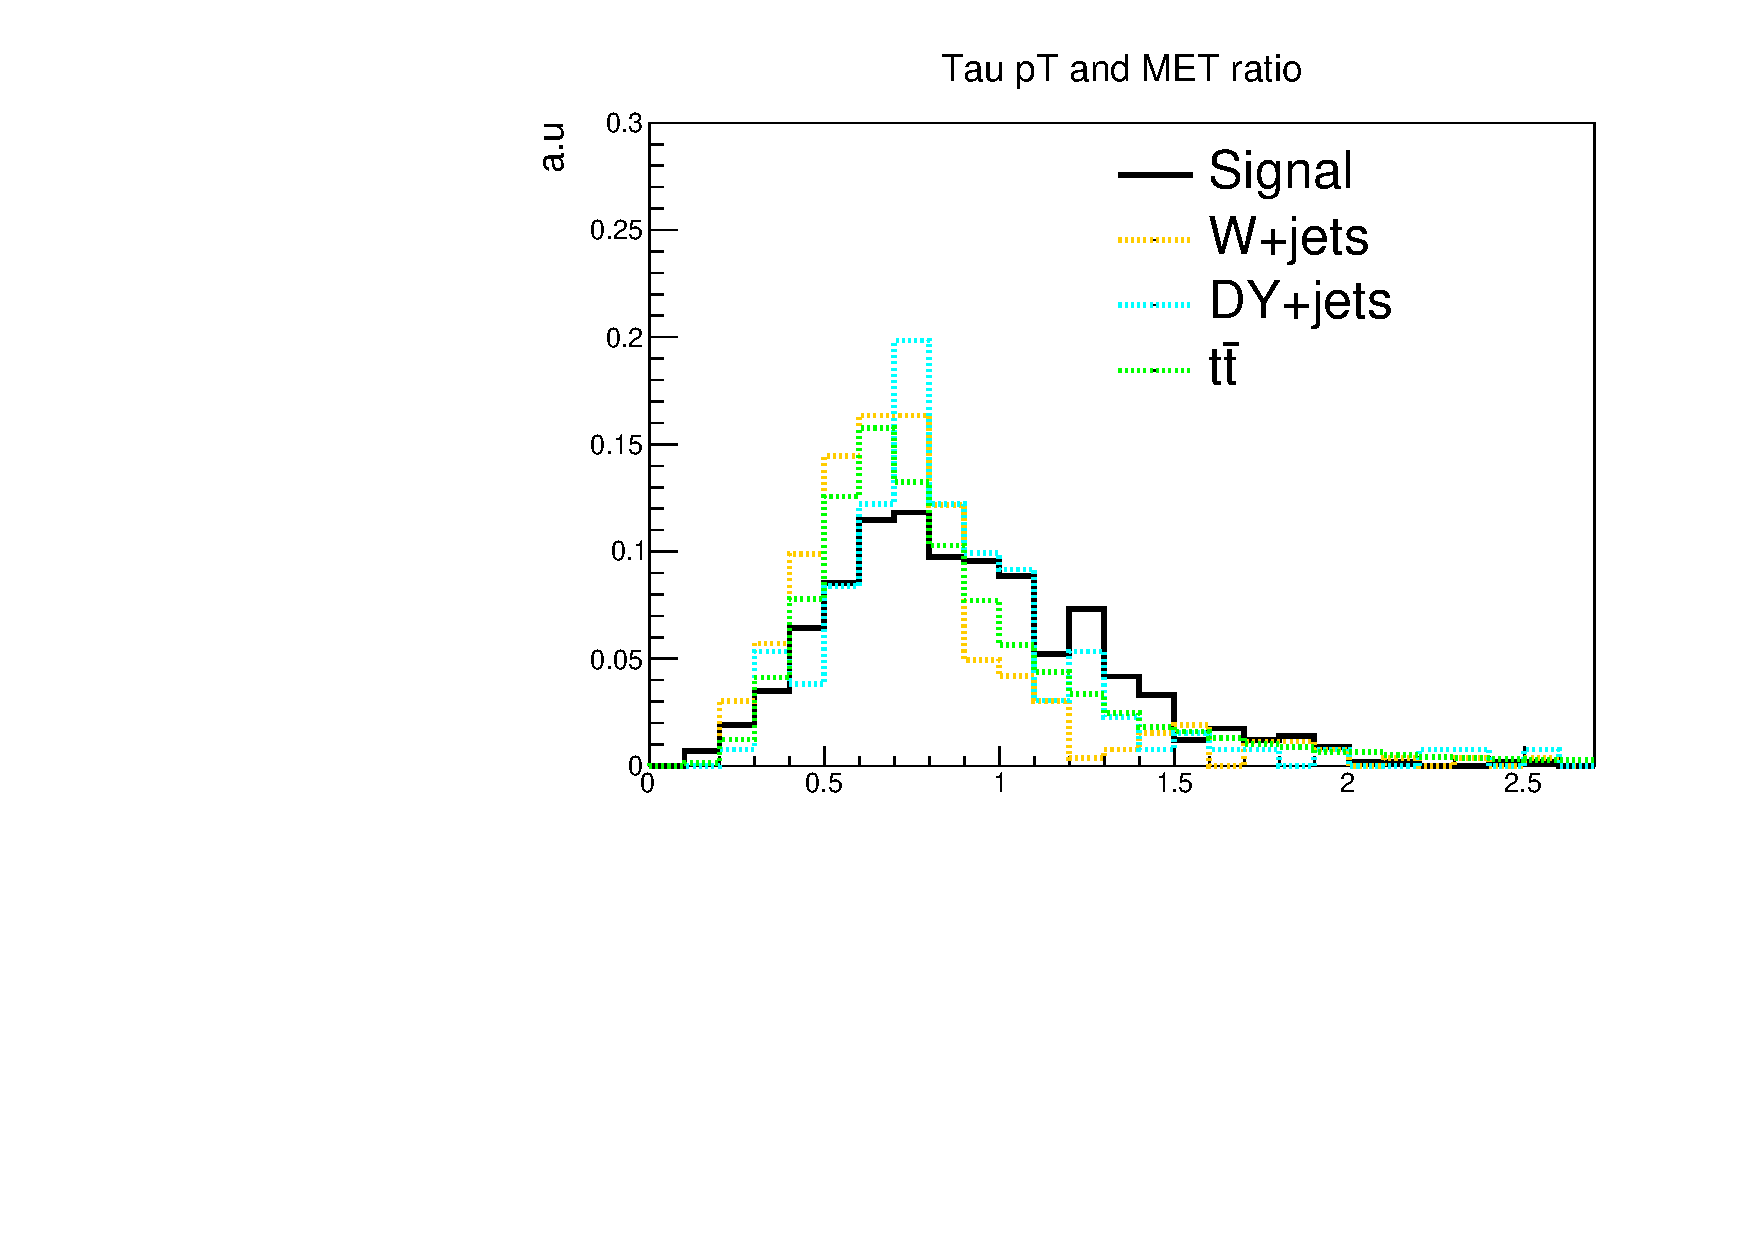
\includegraphics[width = 0.45 \textwidth]{figures/Wp_TauPt_MET_ratio}
\caption{En el grafico se comparan las siguientes distribuciones cinemáticas: $E^{\text{miss}}_{T}$ (superior izquierda), $p^{\tau}_{T}$ (superios derecha) y $\Delta \phi (p^{\tau}_{T}, E^{\text{miss}}_{T})$ (inferior izquierda) y $p^{\tau}_{T}/E^{\text{miss}}_{T}$ (inferior derecha). Para una señal con $M_{W^{\prime}}=500$ GeV y $g_{\tau}=g_{q} = 0.1$ y los backgrounds más dominantes. Las distribuciones están normalizadas a la unidad.}
\label{Fig:DisCine}
\end{center}
\end{figure}
%

Debido a que los electrones cuando atraviesan los tracker de silicio pueden emitir fotones bremsstrahlung energéticos. Los electrón y los fotones generados pueden ser reconstruidos erróneamente como un $\tau_h$. Los muones también se pueden reconstruir como $\tau_h$ cuando decaen en hadrones cargados ($h^{\pm}$). Por lo tanto, para evitar que los canales de electrones ($e^{\pm}$) y muones ($\mu^{\pm}$) en la busqueda del $W^{\prime}$ interfieran, eventos con electrones o muones con $p_T > 15$ GeV no están permitidos. 

Además, debido al decaimiento del $W^{\prime}$ y el $\tau_h$, se tienen dos neutrinos en el estado final, por lo que se espera que los eventos de señal tengan una gran cantidad de $E^{\text{miss}}_T$, en promedio la mitad de la masa del $W'$. Igualmente, dado que para minimizar la incertidumbre en la eficiencia de reconstrucción en el trigger se requiere que $E^{\text{miss}}_{T} > 140$ GeV~\cite{Padeken:2265826}. Finalmente, dada la naturaleza pesada del $W'$ se espera que el ángulo $\phi$ entre el $\tau_h$ y la $E^{\text{miss}}_T$ sea grande. Por lo tanto, $|\Delta \phi (\tau_h, E^{\text{miss}}_T)| > 2.4$ es requerido, lo cual permite eliminar sobre el $85\%$ del background remanente, mientras mantiene la señal por encima del $75\%$(ver fig.~\ref{Fig:DisCine} inferior).

La contribución en el background de los procesos de Cromodinámica cuántica (QCD por sus siglas en inglés) se considera insignificante. Esto para seleccionar al menos un $\tau_h$ con un $p_T$ alto, un jet $b$ y $E^{\text{miss}}_T > 140$ GeV. La tabla~\ref{tab:selections} resume los criterios de selección de eventos usados para el análisis. La figura~\ref{Fig:mTstacked} muestra la distribución de masa transversa entre el $\tau_h$ y $E^{\text{miss}}_T$ para el background y tres diferentes puntos de señal. El background y la señal están normalizados a la producción correspondiente de sección eficaz y a una luminosidad de $100$ fb$^{-1}$.

%
 \begin{figure}
 \begin{center} 
 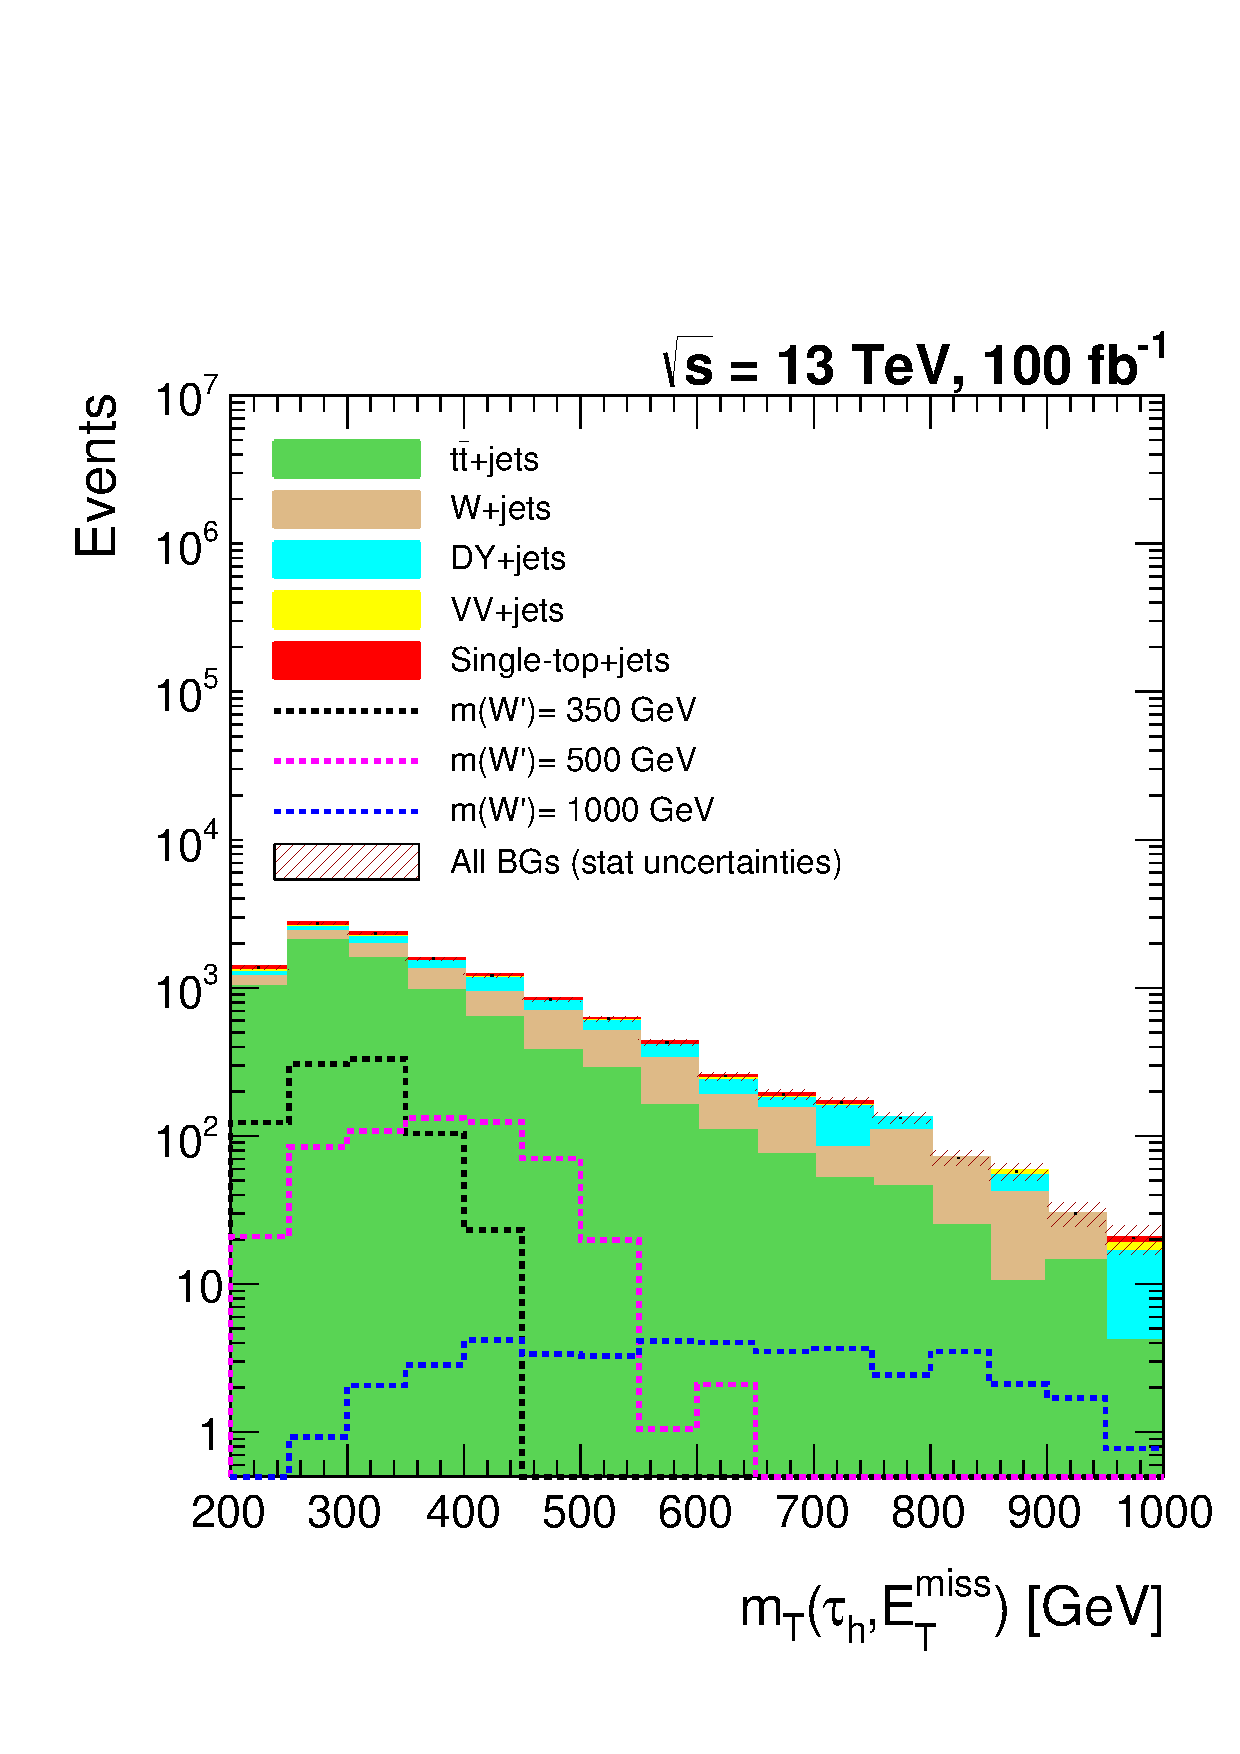
\includegraphics[width=0.5\textwidth]{mT_tauMet.pdf}
 \end{center}
 \caption{Distribución de $m_{T}(\tau_{h},E^{\text{miss}}_{T})$ después de la aplicación de todos los criterios de selección. Los backgrounds se acumulan mientras las señales están superpuestas. Todos los procesos incluidos están normalizados para la sección transversal de producción y la luminosidad de ($100\text{ fb}^{-1}$).}
 \label{Fig:mTstacked}
 \end{figure} 
%

\section{Resultados}\label{sec:results}

Las tablas \ref{tab:cutefficiencySMnew} y \ref{tab:cutefficiencynw} muestran la eficiencia de la selección cinemática basados en la tabla~\ref{tab:selections} y significancia de $100$ fb$^{-1}$ de luminosidad. Se encuentra que la significancia se incrementa con la masa de $W'$ de $200$ GeV a $400$ GeV debido al aumento de la energía faltante en estado final. También se puede notar que el rango de masas de $250$ a $500$ GeV se puede comprobar  usando $100$ fb$^{-1}$ de luminosidad y a nivel de $5\sigma$ cuando $g'_q=g'_\tau=0.1$.

En la figura~\ref{Fig:limits} se muestra una sensitividad proyectada del LHC a $13$ TeV usando este análisis, para $30$, $300$ y $3000$ fb$^{-1}$ de luminosidad en el plano $g'_q-m_{W'}$ superponiendo los ajustes a $1\sigma$ a las medidas de $R(D)$ y $R(D^{*})$ para los diferentes valores de $g'_\tau$. La región por encima de las lines negras tiene una significancia  igual o mayor que $3\sigma$. Gran parte de la banda de mejor ajuste esta al alcance con los datos actuales y la mayor parte de la región restante lo debe estar al final del Run 4.
%
\begin{figure}
\begin{center}
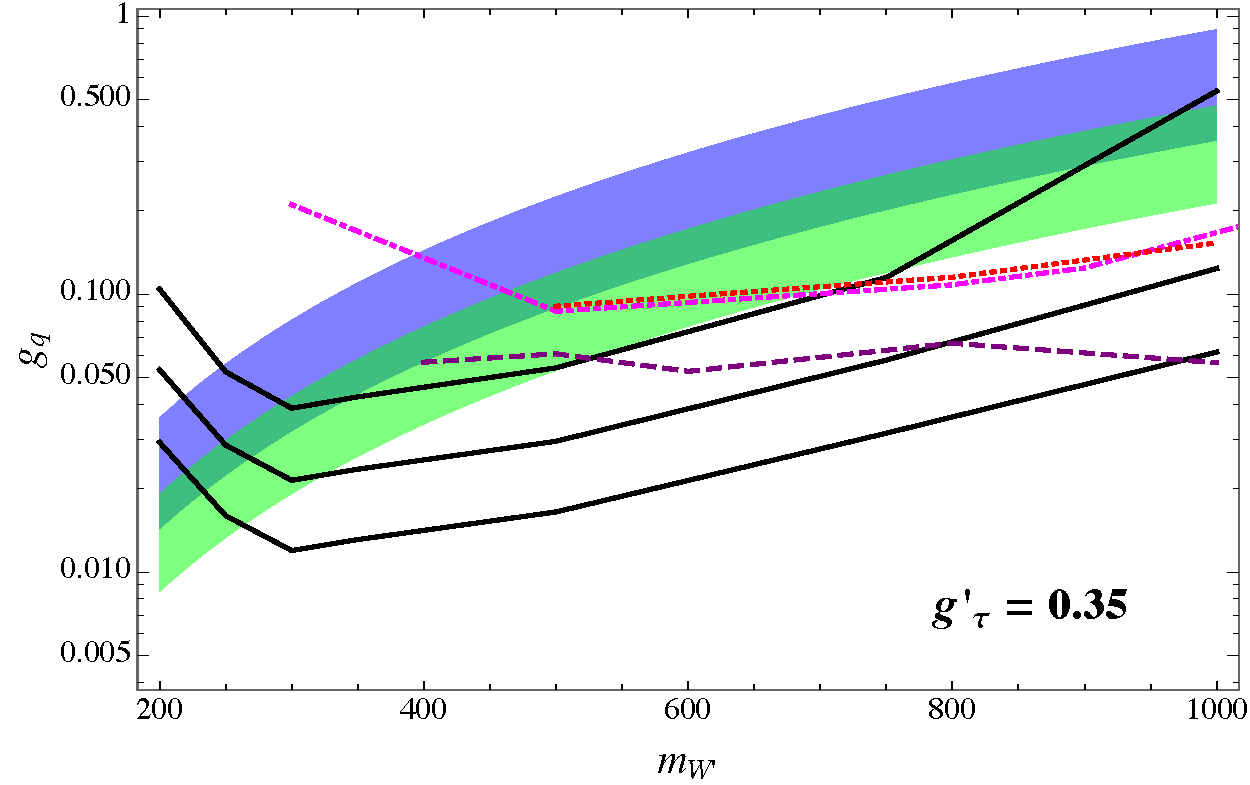
\includegraphics[width = 0.45 \textwidth]{gtau35e2.pdf}
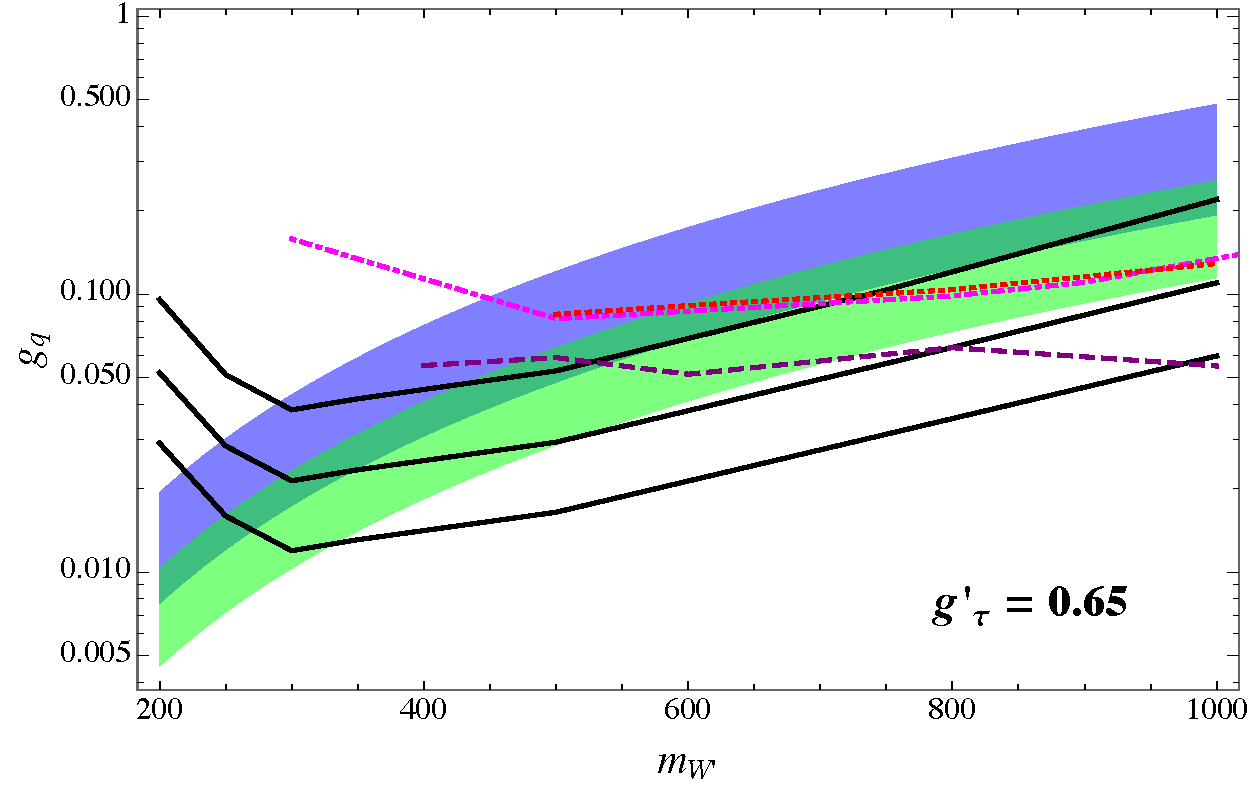
\includegraphics[width = 0.45 \textwidth]{gtau65e2.pdf}
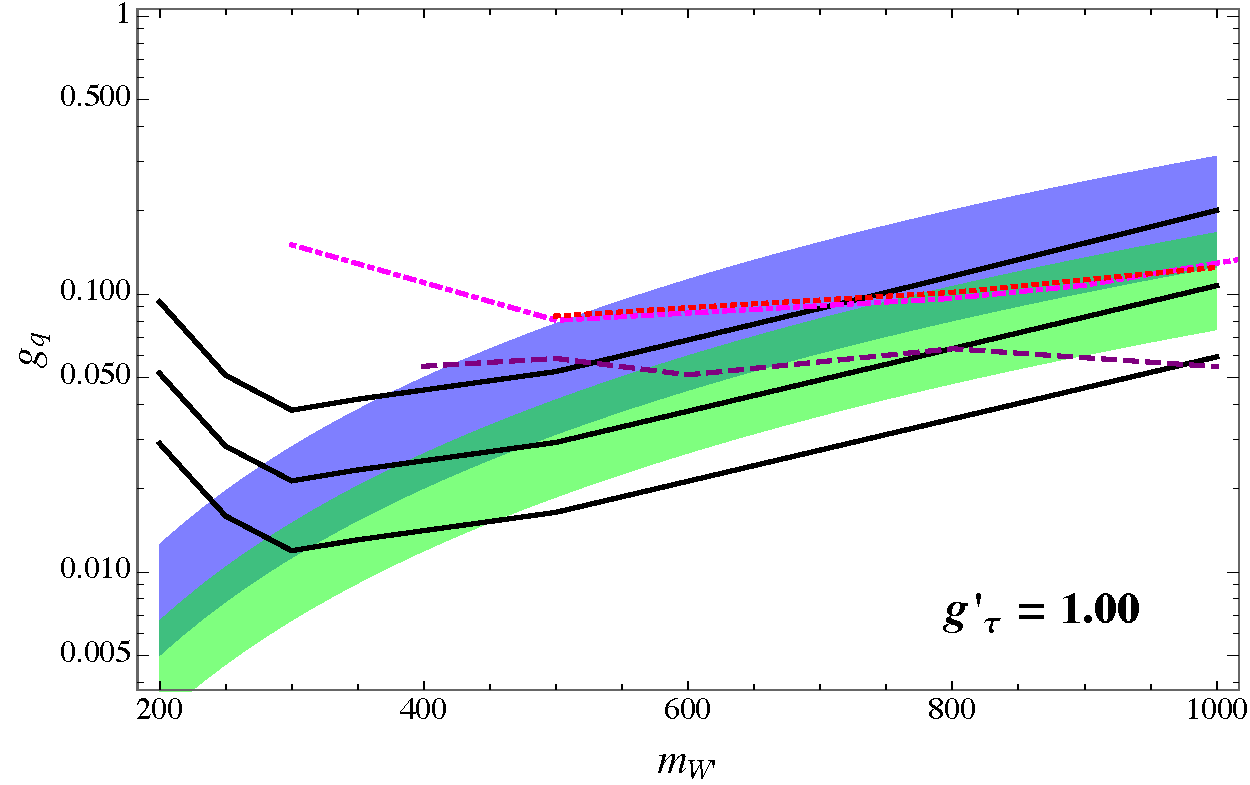
\includegraphics[width = 0.45 \textwidth]{gtau1e0.pdf}
\caption{Sensitividad proyectada a 3$\sigma$ en el acople a los quarks $g'_q$ como función de $m_{W'}$ para $g'_\tau = 0.35\,,0.65\,,1$ en el LHC a 13 TeV y $\mathcal{L}=30\,, 300\,, 3000\, \text{fb}^{-1}$ (curva negra solida) superpuesto con la banda a 1$\sigma$ explicando las medidas de $R(D)$ (azul) and $R(D^\ast)$ (verde). También se muestra los límites inclusivos utilizados por ATLAS a 13 TeV (curva roja punteada) y CMS a 8 TeV (curva magenta punteada).}
\label{Fig:limits}
\end{center}
\end{figure}
%
Note que cuando $g'_{\tau}$ cae por debajo de $0.35$ se comienza a perder la sensitividad debido a los pequeños branching a leptones, y los límites proyectados desaparecen por completo para la luminosidad máxima por debajo de aproximadamente $g'_{\tau} = 0.03$. Cuando $g'_{\tau}$ aumenta, mejora el alcance hasta que los branching a leptones se saturan al $100\%$. Más allá del punto de saturación, los límites no se verán afectados, pero las bandas que están de acuerdo con las anomalías en el mesón $B$ se moveran a valores inferiores de $g'_q$ para compensar. Es importante notar que los límites que se imponen están en los acoplamientos asumidos en la Eq.~\eqref{Eq:LagWp}, los cuales dependen de la teoría completa, podría tener un límite superior comparable a límites aplicados en este trabajo.

También se muestran los límites inclusivos (sin $b$-tag) de la búsqueda de ATLAS utilizando 13 TeV de energía y 36.1 $\text{fb}^{- 1}$ de datos~\cite{Aaboud:2018vgh}, la búsqueda de CMS usando 13 TeV y 35.9 $\text{fb}^{- 1}$~\cite{CMS:2018vff}, y la búsqueda de CMS a 8 TeV con 19.7 $\text{fb}^{- 1}$~\cite{Khachatryan:2015pua}. La búsqueda de 13 TeV de CMS proporciona límites más fuertes que nuestro análisis exclusivo para masas de más de 500 GeV y límites más débiles por debajo de eso. Los límites de ATLAS a 13 TeV, por otro lado, solo comienzan a competir con los límites exclusivos en aproximadamente 700 GeV. Tenga en cuenta que los límites de ATLAS parecen ser significativamente más débiles que los límites de CMS con la misma energía y proporcionan un alcance similar a los límites de CMS a 8 TeV.

\begin{table}[htbp]
\resizebox{17.3cm}{!} {
\begin{tabular}{clllllll}\hline
{} &       $p_T(\tau)$ &             $p_T(b)$ & $e/\mu$ veto & $E_T^{\text{miss}}$ &      $|\Delta \phi (\tau_h,E_T^{\text{miss}})|$ & $N/(\text{100 fb}^{-1})$ \\\hline
$t\bar{t}$    & $3.29 \pm 0.0056$  &   $49.8 \pm 0.087$ &   $71.8 \pm 0.11$ &  $12.4 \pm 0.096$ &  $24.8 \pm 0.36$& $7.41\times 10^{3}$ \\
mono-$t$   & $1.13 \pm 0.0035$ &   $40.4 \pm 0.0035$ &   $90.5 \pm 0.14$ &   $2.55 \pm 0.082$ &   $31.4 \pm 1.5$&$5.95\times 10^{2}$ \\
$W+j$    &   $2.97 \pm 0.0094$ &   $8.4 \pm 0.09$ &   $94.1 \pm 0.26$ &    $9.65 \pm 0.34$ &     $23 \pm 1.6$ &$2.61\times 10^{3}$\\
$Z+j$      &    $2.87 \pm 0.014$ &    $14.1 \pm 0.18$ &   $97.4 \pm 0.21$ &  $6.45 \pm 0.34$ &   $32.4 \pm 2.5$ &$1.37\times 10^{3}$\\
$WW$    & $0.575 \pm 0.0042$ &  $7.66 \pm 0.19$ &    $92.5 \pm 0.7$ &  $6.63 \pm 0.68$ &   $21.6 \pm 4.4$&$3.80\times 10^{1}$ \\
$WZ$     &    $0.638 \pm 0.0071$&  $11.9 \pm 0.36$ &   $93.2 \pm 0.82$ & $6.7 \pm 0.84$ &     $39 \pm 6.3$ &$1.08\times 10^{2}$\\
$ZZ$      &        $0.673 \pm 0.012$&   $17.8 \pm 0.67$ &    $92.7 \pm 1.1$ &     $6 \pm 1$ &   $65.6 \pm 8.4$&$1.77\times 10^{1}$ \\
\hline
&&&&&Total Background&$1.22\times 10^{4}$\\
\end{tabular} }
\caption {Selección de eficiencias en \% y el número total de eventos para 100 fb$^{-1}$ para los procesos de background del ME. Ver el texto y la tabla~\ref{tab:selections} para más detalles.}
\label{tab:cutefficiencySMnew}
\end{table}


\begin{table}[htbp]
\resizebox{17.3cm}{!} {
\begin{tabular}{cllllllll}\hline
{} &               $p_T(\tau)$ &             $p_T(b)$ & $e/\mu$ veto & $E_T^{\text{miss}}$ &      $|\Delta \phi (\tau_h,E_T^{\text{miss}})|$& $N/(\text{100 fb}^{-1})$& $\frac{S}{\sqrt{S+B}}$ \\\hline
200 GeV  &   $8.34 \pm 0.081$ &    $18.1 \pm 0.39$ &   $99.6 \pm 0.15$ &   $5.97 \pm 0.57$ &   $25.7 \pm 4.3$&$1.80\times 10^{2}$& 1.62 \\
250 GeV  &      $13.9 \pm 0.15$ &     $17.2 \pm 0.44$ &  $99.9 \pm 0.078$ &   $15.1 \pm 1$ &     $49 \pm 3.6$ &$5.98\times 10^{2}$&5.30\\
300 GeV  &    $18.3 \pm 0.24$ &     $17.4 \pm 0.56$ &   $99.9 \pm 0.13$ &   $28.6 \pm 1.6$ &   $69.2 \pm 3.1$& $1.06\times 10^{3}$&9.26\\
350 GeV  &    $22.2 \pm 0.27$ &     $17.1 \pm 0.52$ &   $99.7 \pm 0.19$ &   $37.6 \pm 1.6$ &   $67.8 \pm 2.5$&$8.88\times 10^{2}$&7.77 \\
500 GeV  &    $27.5 \pm 0.31$ &     $19.6 \pm 0.52$ &  $99.9 \pm 0.089$ &   $61.5 \pm 1.4$ &   $77.5 \pm 1.6$&$5.63\times 10^{2}$&5.00 \\
750 GeV  &    $31.5 \pm 0.34$ &     $21.7 \pm 0.54$ &   $99.7 \pm 0.16$ &   $79.1 \pm 1.2$ &   $82.4 \pm 1.2$&$1.55\times 10^{2}$&1.40 \\
1000 GeV &   $32.8 \pm 0.37$ &     $21.6 \pm 0.56$ &   $99.7 \pm 0.17$ &   $87.2 \pm 0.98$ &   $83.4 \pm 1.2$&$4.33\times 10^{1}$&0.39 \\\hline
\end{tabular} }
\caption {Selección de eficiencias en \%, y el número total de eventos y significancia para 100 fb$^{-1}$ para la señal en el rango de masas $M_{W'}$ y $g'_q=g'_\tau=0.1$. Ver el texto y la tabla~\ref{tab:selections} para más detalles.}
\label{tab:cutefficiencynw}
\end{table}
%


\chapter*{Conclusiones\markboth{Conclusiones}{Conclusiones}}
\label{sec:Conclusiones}
\addcontentsline{toc}{chapter}{Conclusiones}
\label{Ch:Conclusiones}
Los reporte recientes de las anomalías en los decaimientos del mesón $B$ medidos en Babar, Belle y LHCb pueden ser explicados adicionando un bosón gauge $W'$ al ME, el cual preferencialmente se acople a la tercera generación de fermiones. En este trabajo se estudian las corrientes y posibles señales en la busqueda y detección futura del $W'$ en un modelo simplificado, en el cual el $W'$ solo se acopla a los quarks $b$ y $c$ y al sabor leptónico $\tau$, el cual es responsable de la corriente cargada $b \to c \tau \nu$ que explica los excesos en $R(D)$ y $R(D^*)$~\cite{Abdullah:2018ets}. Mediante los procesos de fusión de $g c$, $g g$ y $c b$, se puede producir un $W'$ que no se acople a la primera generaicón de  fermiones.

Estos nuevos procesos de producción del $W'$ pueden conducir a un jet $b$ junto con $\tau+\nu$ de estado final, lo cual nos permite usar un nuevo estado final exclusivo $b+\tau_h+E^{miss}_T$ reportado aquí para la busqueda del $W'$ en el LHC. El estudio detallado del background y la señal muestran que la presencia de el jet $b$ en el estado final exclusivo es bastante efectivo para reducir el background del ME. Además, la aparición de un jet $b$ en el estado final establecería el acoplamiento del $W'$ con los fermiones de tercera generación, lo cual es crucial para dar explicación de la anomalía.

Los análisis inclusivos de CMS y ATLAS muestran una restricción para la masa del $W^\prime$ por encima de 300 GeV y 500 GeV, respectivamente. Sin embargo, utilizando los cortes desarrollados en nuestro estudio demostramos que el alcance puede mejorarse para el rango de masa 200-500 GeV. Igualmente, se muestra que el rango de masas de 250-500 GeV puede probarse a nivel de $\sim 5 \sigma$ con una luminosidad de 100 fb$^{- 1}$ para $g_b = 0.1$ y $g_\tau = 0.1$. Consecuentemente, una región amplia del espacio de parámetros que explica las anomalías puede ser investigada directamente en el LHC. Los resultados del análisis aquí presentado pueden ser aplicados a un modelo con un $W'$ con canales de decaimiento adicionales después de aplicar un factor de escala adecuado, derivado de los branching de $W'$. 

%
% Appendices
	\appendices
\chapter{Generando UFO files con \textsc{FeynRules}}\label{GenUFO}

Para cargar un modelo en \textsc{FeynRules} se debe cargar el paquete en una sesión de \textsc{Mathematica}. Esto debe hacerse antes de que la descripción del modelo se cargue en el kernel, por lo que debe ser la primera línea del notebook de \textsc{Mathematica}. Para cargar \textsc{FeynRules}, el usuario primero debe especificar el directorio donde está almacenado y luego cargarlo usando 
%
\begin{verbatim}
$$ FeynRulesPath = SetDirectory[<La direccion del paquete>];
<< FeynRules'
\end{verbatim}
%
Por ejemplo, si el paquete se encuentra en el \verb|/home| se usa:
%
\begin{verbatim}
$$ FeynRulesPath = SetDirectory["~/feynrules-directorio"];
<< FeynRules'
SetDirectory["~/feynrules-directorio/Models/"];
\end{verbatim}
%
El \verb|SetDirectory| hace referencia a la ubicación donde buscará el modelo en el momento de cargarlo. Después de cargar el paquete de \textsc{FeynRules}, se puede cargar el modelo usando el comando 
%
\begin{verbatim}
LoadModel[<archivo.fr>, <archivo2.fr>, ...];
\end{verbatim}
%
Para que \textsc{FeynRules} corra adecuadamente, la extensión de los archivos debe ser \textbf{.fr}. \textsc{FeynRules} tiene la ventaja de poder almacenar el modelo en un solo archivo o en varios. Por ejemplo, si se quiere hacer una extensión al Modelo Estándar solo es necesario agregar el archivo adicional que genere la extensión. De esta forma el modelo se carga así:
%
\begin{verbatim}
LoadModel["sm.fr", "WZPrime.fr"];
\end{verbatim}
%
Cada vez que el modelo cambie, se debe volver a cargar.
Ahora, ya que se tiene cargado el modelo, \textsc{FeynRules} posee una variedad de comandos que permiten obtener los vértices, las reglas de Feynman asociados al lagrangiano, los parámetros del modelo, etc.  Dichos comandos y una descripción más detalladas se pueden encontrar en~\cite{Alloul:2013bka}. 

Una vez se han obtenido las reglas de Feynman, el usuario generalmente está interesado en la fenomenología del modelo, que requiere la evaluación de los diagramas de Feynman. Hay muchas herramientas que permiten evaluar diagramas de Feynman automáticamente. Si bien estas herramientas son en general muy flexibles y permiten al usuario generar, al menos en principio, diagramas de Feynman para cualquier proceso que satisfaga los requisitos básicos de la teoría cuántica de campos, la mayoría de las herramientas requieren una trabajo tedioso y propenso a errores para la implementación de estos.

\textsc{FeynRules} da la posibilidad de obtener salidas para varias interfaces. Actualmente \textsc{FeynRules} genera salidas para las siguientes interfaces,
\begin{itemize}
\item CalcHep/CompHep
\item FeynArts/FormCalc
\item Sherpa
\item UFO (Universal FeynRules output)
\item Whizard/Omega
\end{itemize}

El formato UFO es un formato de modelo genérico que almacena información del modelo de forma abstracta en forma de objetos Python para \textsc{MadGraph}. Todas las interfaces pueden ser invocadas con el comando 
%
\begin{verbatim}
WriteXOutput[L 1 ,L 2 ,. . . , options];
\end{verbatim}
%
donde $X$ es reemplazado con la etiqueta de referencia al nombre de cada interfaz. Las principales limitaciones de las interfaces se basan en el hecho de que solo se pueden usar para implementar partículas y vértices que son compatibles nativamente con el generador de diagramas de Feynman correspondiente. Ya que cada generador realiza suposiciones implícitas sobre las rotaciones o las representaciones de color de las partículas presentes en el modelo, y / o sobre la forma o la dimensión de los vértices de interacción. Como consecuencia, solo aquellos modelos que cumplen con todas esas restricciones son compatibles con una herramienta determinada. Las interfaces de \textsc{FeynRules} se adaptan a los diferentes generadores de diagramas de Feynman y, por lo tanto, permiten verificar caso por caso si un modelo dado cumple o no con una herramienta determinada. Por ejemplo, si una interfaz detecta que un vértice de interacción determinado no es compatible, el vértice se descarta y se imprime una advertencia en la pantalla. El usuario tiene la posibilidad de cambiar a un generador de diagramas Feynman diferente para el cual la restricción no está presente.

Si el interés es generar los UFO files necesarios para correr en \textsc{MadGraph} se debe ejecutar el siguiente comando
%
\begin{verbatim}
WriteUFO[<Lag1>, <Lag2>, …, Output -> "Carpeta", opciones];
\end{verbatim}
%
donde recibe como parámetros de entrada el lagrangiano de los diferentes archivos cargados en el notebook de \textsc{Mathematica}y la carpeta donde se quiere depositar los UFO files. En general se ejecuta  
%
\begin{verbatim}
WriteUFO[LFull, Output -> "UFO_files_output"];
\end{verbatim}
%
Tenga en cuenta que para que los archivos UFO funcionen correctamente, se debe asignar a todas las constantes de acoplamiento una orden de interacción.. En general se ejecuta
\newpage
\chapter{Modelo en \textsc{FeynRules}}\label{FeynRModel}
La implementación del modelo en \textsc{FeynRules} es:
\begin{verbatim}
(* ********************************************************* *)
(* *****                                               ***** *)
(* *****  FeynRules model file: SM + W&Z prime	       ***** *)
(* *****  Original Author:  M. Abdullah                ***** *)
(* *****                                               ***** *)
(* ********************************************************* *)

(* ************************** *)
(* *****  Information   ***** *)
(* ************************** *)
M$ModelName = "WZPrime";
M$Information = { Authors->{"M. Abdullah"}, 
		  Emails->{"mabdullah@tamu.edu"}, 
		  Institutions->{"Texas A&M University"},
          Date->"2017 Jan 11", 
		  Version->"1.0"};
FeynmanGauge = True;

(* ************************** *)
(* *****     Fields     ***** *)
(* ************************** *)
M$ClassesDescription = {
(* W prime boson *)
  V[34] == {
	ClassName        -> Wp,
	SelfConjugate    -> False,
	Mass             -> {MWp,  500.00},
	Width            -> {WWp,    50},
	ParticleName     -> "Wp+",
	AntiParticleName -> "Wp-",
    QuantumNumbers   -> {Q -> 1},
	PDG              -> 34, 
	PropagatorLabel  -> "Wp",
	PropagatorType   -> Sine,
	PropagatorArrow  -> None,
	FullName         -> "Wp"
  },

(* Z prime boson *)
  V[32] == {
	ClassName        -> Zp,
	SelfConjugate    -> True,
	Mass             -> {MZp,  500.00},
	Width            -> {WZp,    50},
	ParticleName     -> "Zp",
	PDG              -> 32, 
	PropagatorLabel  -> "Zp",
	PropagatorType   -> Sine,
	PropagatorArrow  -> None,
	FullName         -> "Zp"
  }
};

(* ************************** *)
(* *****   Parameters   ***** *)
(* ************************** *)
M$Parameters = {
  gb == { ParameterType -> External, 
	  Value -> 0.1,
	  InteractionOrder -> {BSM, 1},
	  BlockName->ZprimeCouplings,
	  TeX -> Subscript[g,b], 
          Description -> "Z' coupling to 3rd gen quarks"
	},

  gmu == { ParameterType -> External, 
	  Value -> 0.1,
	  InteractionOrder -> {BSM, 1}, 
	  TeX -> Subscript[g,mu], 
	  BlockName->ZprimeCouplings,
          Description -> "Z' coupling to 2nd gen leptons"
	},
	
	gtau == { ParameterType -> External, 
	  Value -> 0.1,
	  InteractionOrder -> {BSM, 1}, 
	  TeX -> Subscript[g,tau], 
	  BlockName->ZprimeCouplings,
          Description -> "Z' coupling to 3rd gen leptons"
	},
	
	delbs == { ParameterType -> External, 
	  Value -> 1.0,
	  InteractionOrder -> {BSM, 0}, 
	  TeX -> Subscript[delta,bs], 
	  BlockName->ZprimeCouplings,
          Description -> "Z' coupling scale factor to b and s quarks"
	},
	
	gwp == {ParameterType -> External,
	Value -> 0.1,
	InteractionOrder -> {BSM,1},
	TeX -> Subscript[g,wp],
	Description -> "W' coupling",
	BlockName->WprimeCoupling,
	Description-> "W' coupling"
	},
	
	Vcb == { ParameterType -> Internal,
	Value -> 0.0412,
	InteractionOrder -> {BSM,0},
	TeX -> Subscript[V,cb],
	Description -> "c-b CKM mixing"
	}

};

(* ******************************* *)
(* *****   BSM Lagrangians   ***** *)
(* ******************************* *)

LZQ := gb*Zp[mu]*( tbar.Ga[mu].ProjM.t \
			   +  bbar.Ga[mu].ProjM.b \
			   + delbs*sbar.Ga[mu].ProjM.b \
			   +HC[delbs*sbar.Ga[mu].ProjM.b]);
			   
LZL := 			gmu*Zp[mu]*(mubar.Ga[mu].mu \
				+vmbar.Ga[mu].ProjM.vm)\
				+gtau*Zp[mu]*(tabar.Ga[mu].ta \
				+vtbar.Ga[mu].ProjM.vt);
				
LW  := gwp*(Wp[mu]*cbar.Ga[mu].ProjM.b \
		+HC[Wp[mu]*cbar.Ga[mu].ProjM.b] \
		+Wp[mu]*vtbar.Ga[mu].ProjM.ta \
		+HC[Wp[mu]*vtbar.Ga[mu].ProjM.ta]);

(* Combine Everything *)

LFull := LSM + LZQ + LZL + LW;
\end{verbatim}
\newpage
\chapter{Generación de eventos en \textsc{MadGraph}}\label{GenMG}
Para cargar un modelo en \textsc{MadGraph}, primero se debe certificar que la carpeta con los archivos UFO se encuentre en la carpeta \textsc{models}. Luego se debe ejecutar el comando 
%
\begin{verbatim}
MG5_aMC> import model [directorio_del_modelo]
\end{verbatim}
%
Después de esto se deben de definir los eventos a generar. Se comienza definiendo los estados iniciales en el evento, separados de los estados finales por “\textgreater”. Para generación de procesos partónicos se utiliza el comando 
%
\begin{verbatim}
MG5_aMC> generate p p > S
\end{verbatim}
%
donde $S$ hace referencia a todas las partículas en el estado final, sin incluir partones ligeros de QCD, ni quarks b (y que no incluye partículas BSM cargadas bajo QCD). Si se desea adicionar procesos a la generación de eventos se ejecuta el siguiente comando
%
\begin{verbatim}
MG5_aMC> add process p p > S1
\end{verbatim}
%
donde $S1$ hace referencia a un conjunto diferentes de partículas en el estado final anterior.
Además, si se quiere adicionar jets ($j$), sólo se necesita adicionar $j$ a los estados finales. Por ejemplo, para adicionar eventos con dos jets se ejecuta el siguiente comando
%
\begin{verbatim}
MG5_aMC> add process p p > S j j
\end{verbatim}
%
Luego de tener los procesos para generar los eventos, se debe almacenar la salida de dichos eventos para la ejecución. Para esto se ejecuta el comando
%
\begin{verbatim}
MG5_aMC> output [directo_de_salida] -f
\end{verbatim}
%
Si el directorio no existe lo crea, de lo contrario, si el directorio existe la bandera \verb|-f| se utiliza para borrar todos los archivos en estos. 

Antes de realizar la ejecución se deben definir los diferentes parámetros de la generación de eventos. En \textsc{MadGraph} los parámetros se configuran de las tarjetas de configuración. Todas éstas tarjetas de configuración se pueden encontrar en el directorio \verb|Cards| en el directorio de salida generado por \textsc{MadGraph}. La \verb|proc_card|, es dónde se declaran los procesos a generar. Esta tarjeta se genera automáticamente y su modificación no tiene efecto alguno. La \verb|param_card|, es la tarjeta donde se controla el valor de los parámetros del modelo. La \verb|run_card|, permite controlar los parámetros de la simulación, por ejemplo, el número de eventos a generar.

Luego de tener la configuración que se desea, se deben ejecutar los procesos anteriormente generados. Para esto se utiliza el comando
%
\begin{verbatim}
MG5_aMC> launch [directo_de_salida]
\end{verbatim}
%
Después de esto vemos la interfaz de MadGraph~\ref{Fig:IMG}, donde preguntan por los programas para las diferentes simulaciones de los procesos. 
%
\begin{figure}
\begin{center}
\begin{verbatim}
The following switches determine which programs are run:
/--------------------------------------------------------------------------------\
|  1. Choose the shower/hadronization program:           shower = PYTHIA8      |
|  2. Choose the detector simulation program:            detector = OFF        |
|  3. Run an analysis package on the events generated:   analysis = No analysis 
tool interfaced to MG5aMC.|
|  4. Decay particles with the MadSpin module:		      	   madspin = OFF         |
|  5. Add weights to events for different model hypothesis:		   reweight = OFF              |
/--------------------------------------------------------------------------------\
\end{verbatim}
\caption{Interfaz de MadGraph. Se preguntan por los programas requeridos para simulaciones requeridas en los procesos.}
\label{Fig:IMG}
\end{center}
\end{figure}
%
Para realizar la simulación del proceso de hadronización sobre el proceso partónico se utiliza Pythia 8. 

Para realizar simulaciones con jets adicionales se debe de realizar el proceso de \textbf{merging}. Este proceso consiste de la separación del espacio de parámetros que es simulado por \textsc{MadGraph} y por Pythia. \textsc{MadGraph} debe encargarse solo de los jets “duros” (con gran cantidad de momento) y Pythia se debe encargar de los jets “suaves” (con baja cantidad de momento). Para garantizar el \textbf{merging} se deben definir los valores de \textbf{xqcut} para MadGraph y \textbf{qcut} Pythia. 

Para encontrar los valores óptimos de las variables de \textbf{merging}, para cada valor de \textbf{xqcut} se debe realizar un escaneo sobre \textbf{qcut} (teniendo en cuenta que \textbf{xqcut} \textless \textbf{qcut}) hasta encontrar el valor que estabilice la sección eficaz. La optimización cambia de acuerdo a los procesos, el número de jets adicionales incluidos y/o los cortes cinemáticos.

\chapter{Comparación LO vs NLO}\label{LOvsNLO}

\begin{table}[htbp]
\begin{center}
\begin{tabular}{clll}\hline
$M_{W^{\prime}}$ [GeV] &               $\sigma_{LO}$ [Pb] &             $\sigma_{NLO}$ [Pb] & Cambio relativo \\\hline
200  &   $30.38$ &    $35.07 $ &    $15.43\%$ \\
700 &    $0.1654$ &   $0.1796 $ &   $8.58\%$ \\
1000 &   $0.02603$ &  $0.02778 $ &  $6.7\%$ \\\hline
\end{tabular}
\caption {Comparación de sección eficaz para procesos generados a orden principal (LO) y a segundo orden (NLO).}
\label{tab:cutefficiencynw}
\end{center}
\end{table}
%


%
\begin{figure}
\begin{center}
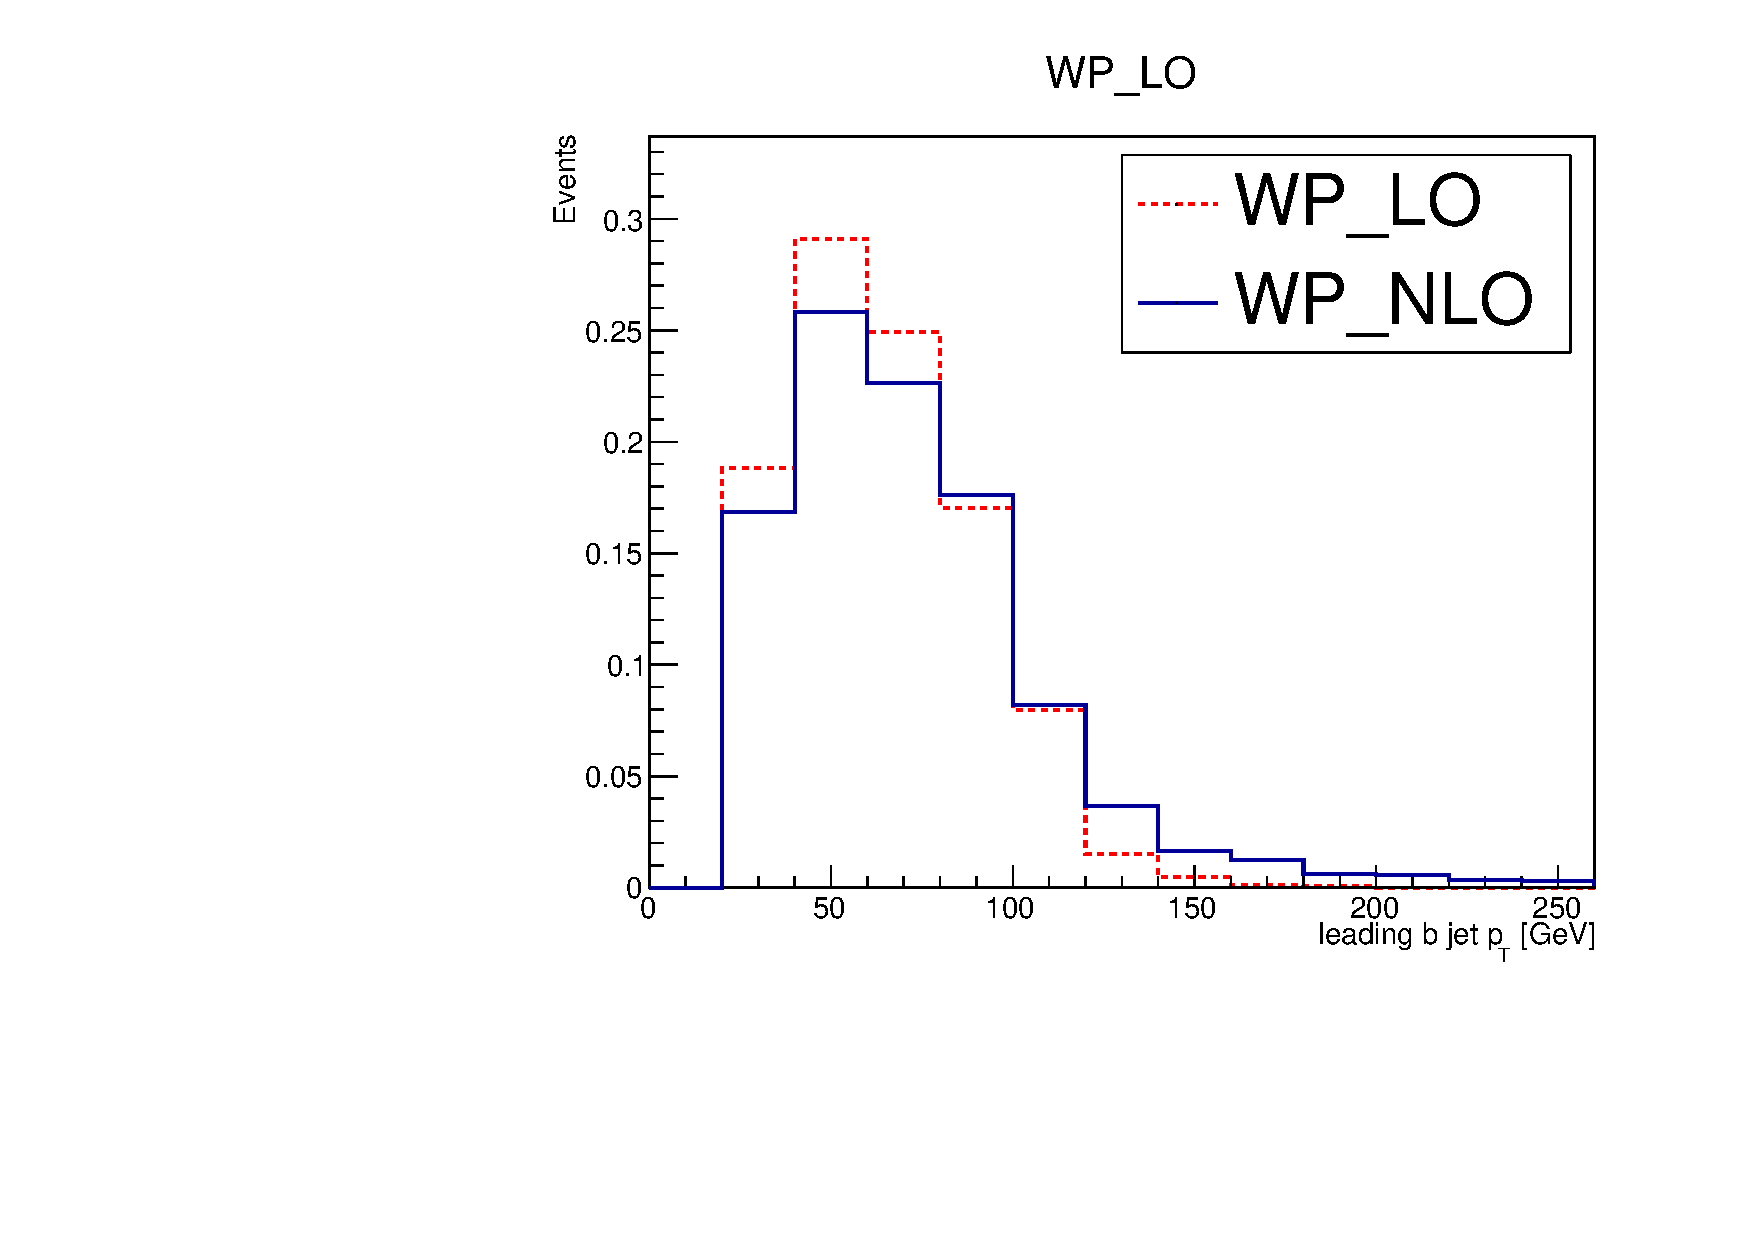
\includegraphics[width = 0.45 \textwidth]{figures/leading_jet_p_T_200_Norm.pdf}
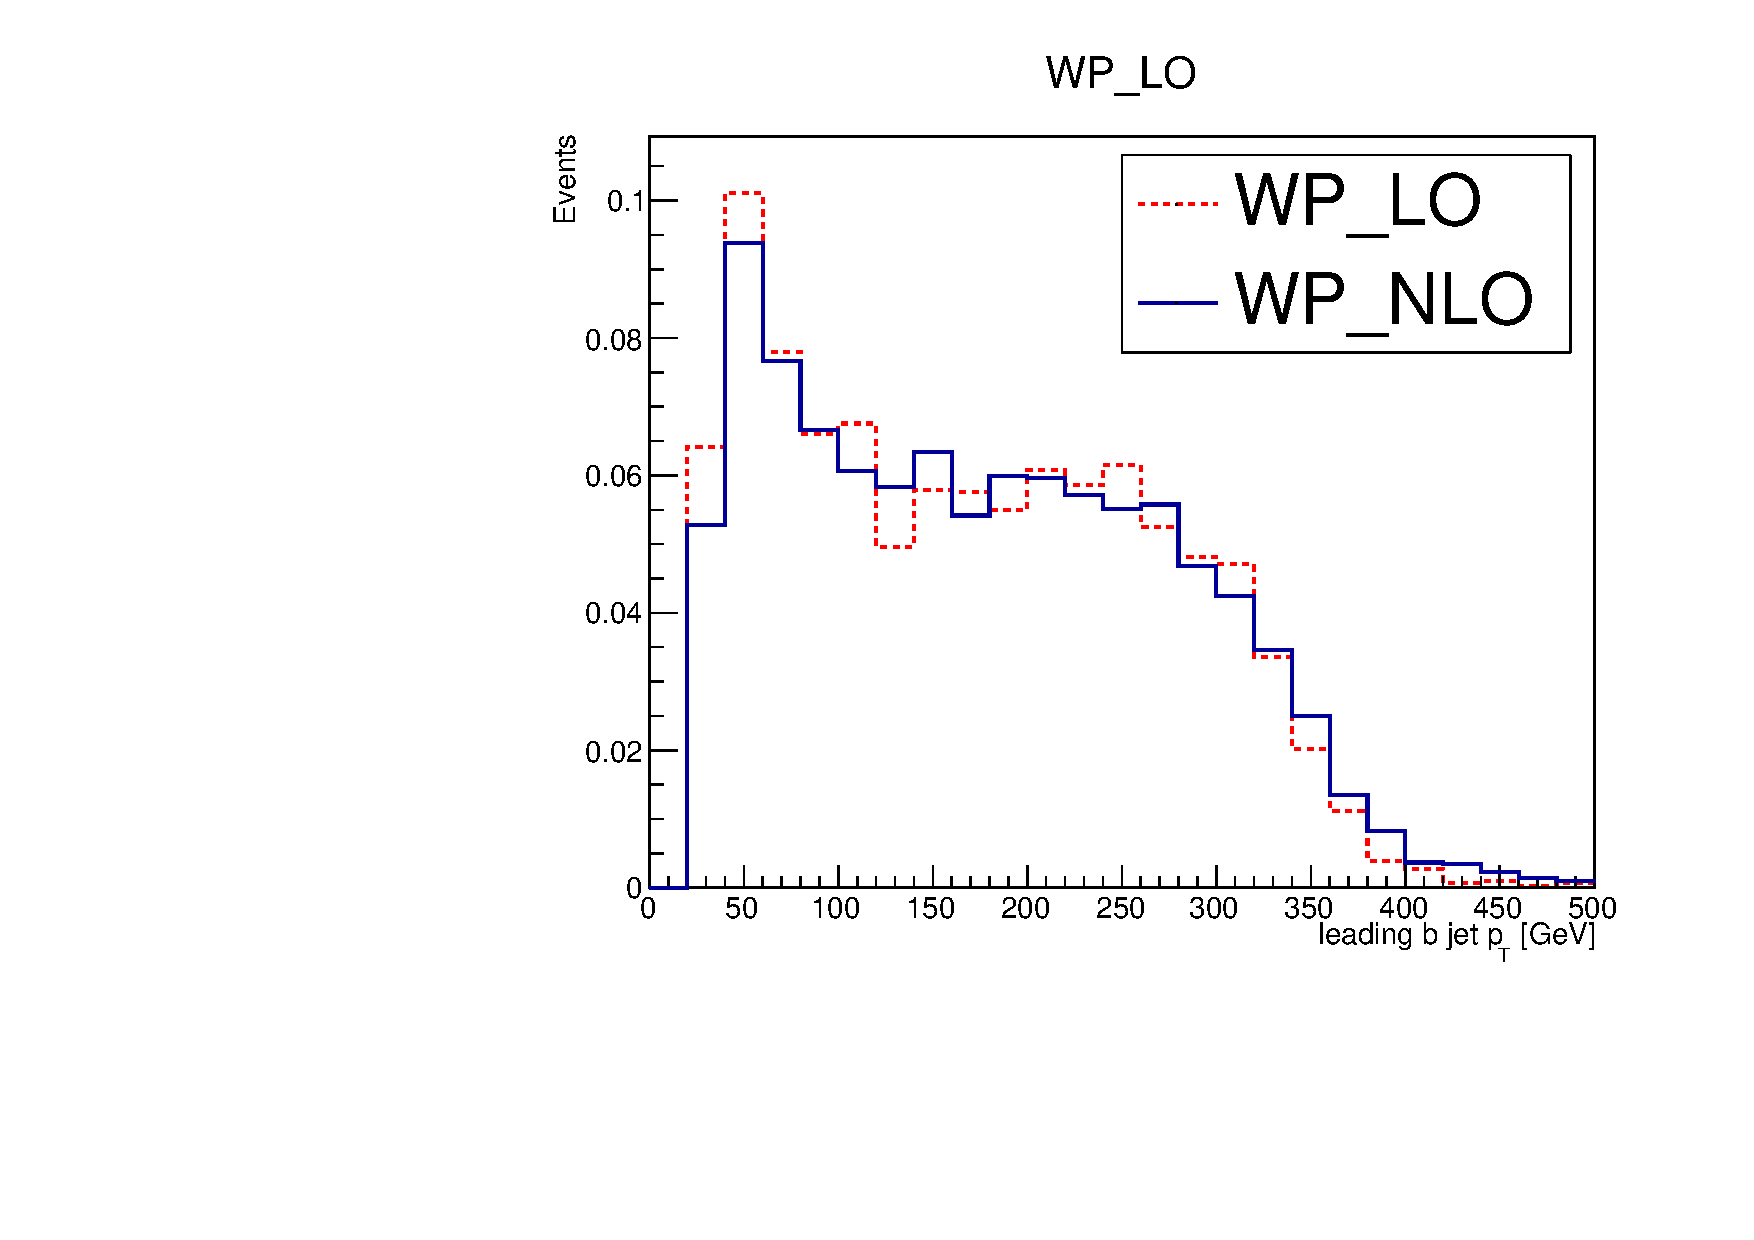
\includegraphics[width = 0.45 \textwidth]{figures/leading_jet_p_T_700_Norm.pdf}
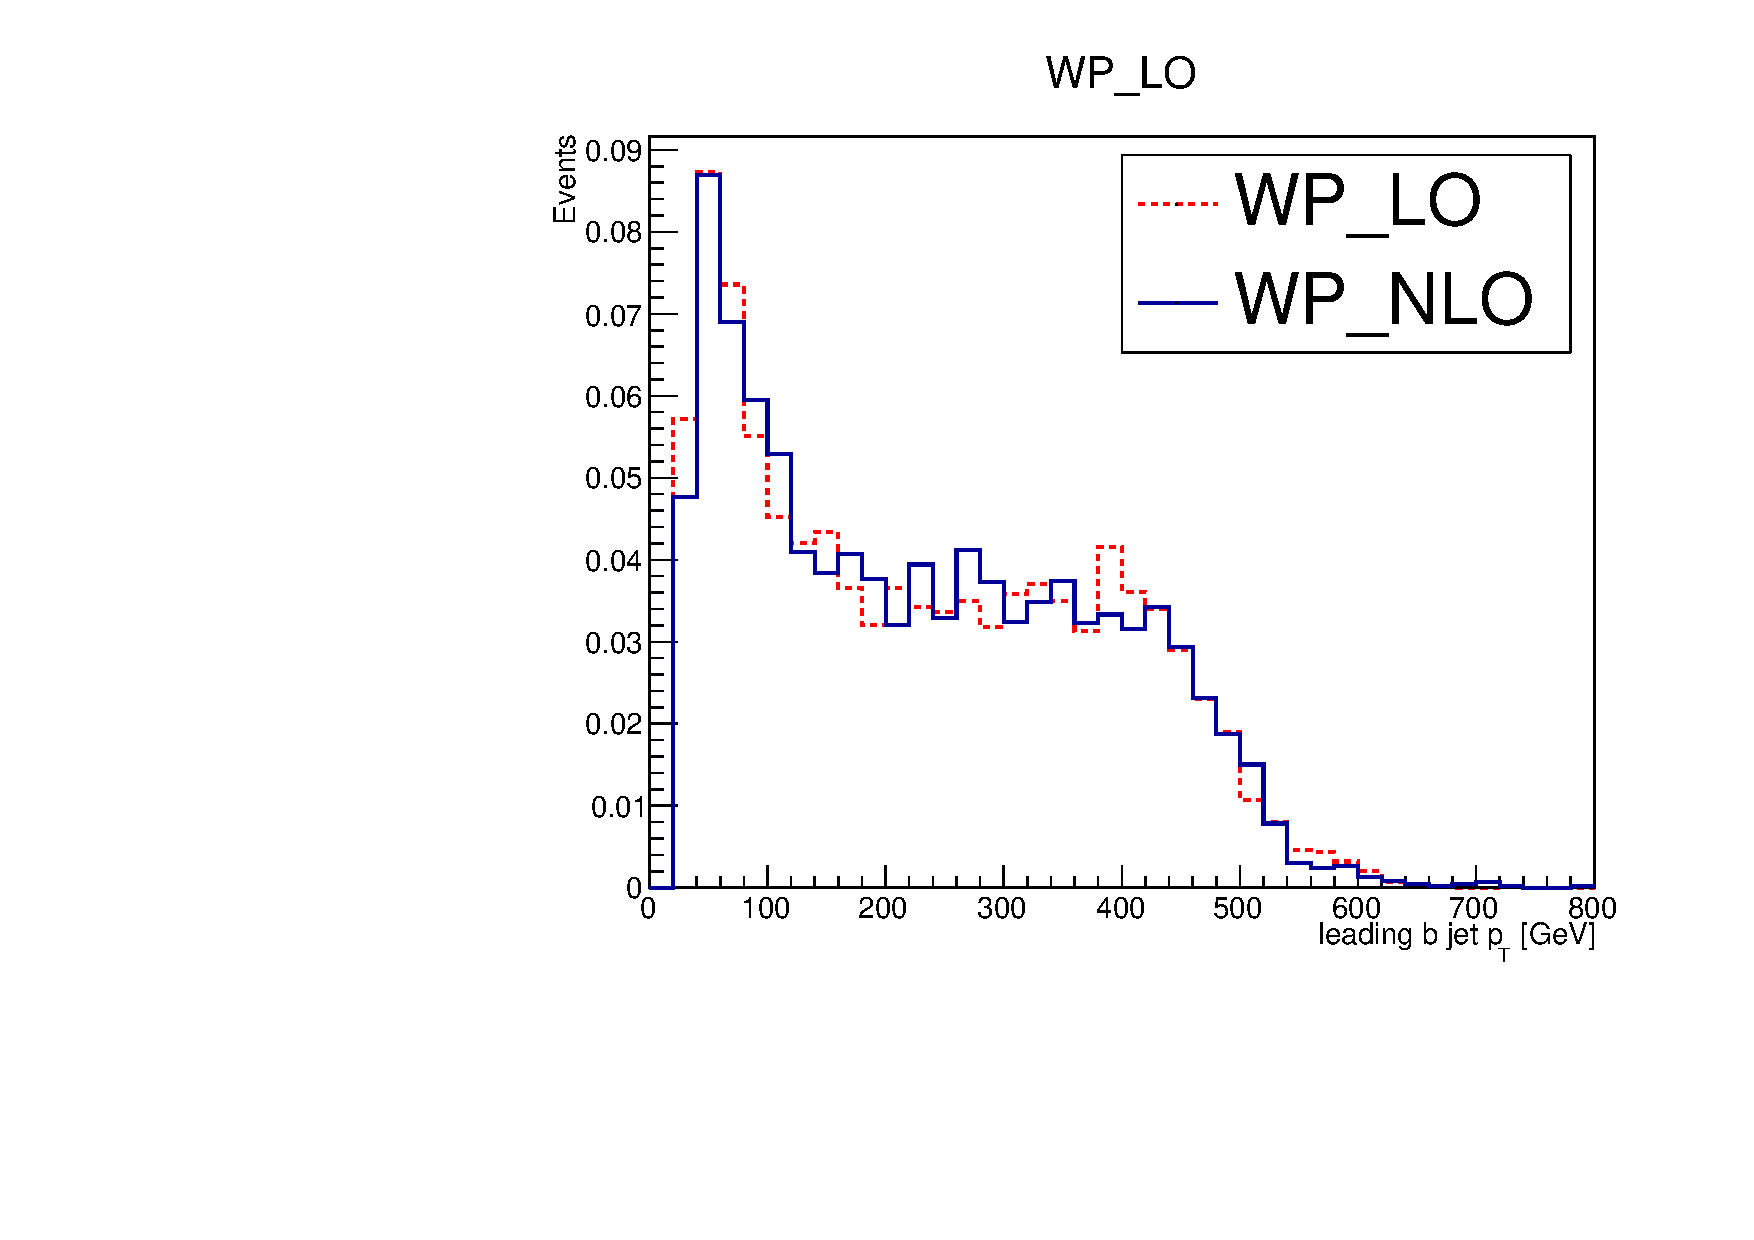
\includegraphics[width = 0.45 \textwidth]{figures/leading_jet_p_T_1000_Norm.pdf}
\caption{Distribución de $p_{T}$ para el jet $b$ principal para $M_{W^{\prime}} = 200$ GeV (superios izquierda), $M_{W^{\prime}} = 700$ GeV (superior derecha) y $M_{W^{\prime}} = 1000$ GeV (inferior). Aquí no se ve un cambio significativo en la distribución de $p_{T}$ para los eventos simulados a orden principal (LO) y a segundo orden (NLO).  }
\label{Fig:DisCine}
\end{center}
\end{figure}
%
%
% Acknowledgements (content in `acknowledgements.tex')
%%%%%%%%%%%%%%%%%%%%%%%%%%%%%%%%%%%%%%%%%%%%%%%%%%%%%%%%%%%%%%%%%%
%%
%% use the starred version of the "acknowledgements" environment
%% to omit signatures from this section, e.g.:
%% \begin{acknowledgements*} ... \end{acknowledgements*}
%% 
%%%%%%%%%%%%%%%%%%%%%%%%%%%%%%%%%%%%%%%%%%%%%%%%%%%%%%%%%%%%%%%%%
\begin{acknowledgements}

I would like to thanks all the people that in some way have helped me with the elaboration of this thesis.

First, I would like to thanks ....
\end{acknowledgements}
	
%
%%%%% Bibliography/References (BiBTeX items in `references.bib')
%%%%	\bibliography{IEEEabrv,references}
%\bibliographystyle{jhep}
\bibliographystyle{apsrev4-1long}
\bibliography{BibliMSc}
% Abbreviations (content in `abbreviations.tex') 
	%\includeabbreviations{abbreviations}
% Glossary (content in `glossary.tex') 
	%\includeglossary{glossary}
%%%%%%%%%%%%%%%%%%%%%%%%%%%%%%%%%%%%%%%%%%%%%%%%%%%%
% Index
	%\printindices
%
%%%%%%%%%%%%%%%%%%
%%%%%%%%%%%%%%%%%%

%% Create CD labels:

	\definecdlabeloffsets{0}{-0.65}{0}{0.55} % upper label x offset [cm] (default=0) /  upper label y offset [cm] (default=0) /  lower label x offset [cm] (default=0) /  lower  label y offset [cm] (default=0) -- For Q-Connect KF01579 labels use the following offset values: {0}{-0.65}{0}{0.55}

	\createcdlabel{This is my PhD \\ Super title}{Juan Valdez}{October}{2016}{1} % thesis title / author name / month / year / title area width in cm (recommended value: 8) 

%%
%% Create CD case covers:

	\createcdcover{This is my PhD \\ Super title}{Juan Valdez}{October}{2016}{1} % thesis title / author name / month / year / title area width in cm (recommended value: 10) 

%%
%
\end{document}

%%%%%%%%%%%%%%%%%%%%%%%%%%%%%%%%%%%%%%%%%%%%%%%%%%%%